\chapter{Second quantization}

Fock space allows us to effectively encode systems of $A$ nucleons  by considering only the occupancy of various
single-particle states. In quantum mechanics all particles are indistinguishable, and in the same Fock 
space all particles are identical. To describe quantum mechanical states of many particles, we take the tensor product 
of as many different Fock spaces as there are species of particles under consideration. 
It is one of the most powerful features of the Fock space formalism  that states are intrinsically properly symmetrized. 

A useful and convenient basis for this space is the occupancy number basis. 
If $|\Phi_{\lambda}\rangle$ forms a  basis of our Hamiltonian, 
then we can construct a Slater determinant (we limit ourselves to fermions) as
\be
|\Phi_{\lambda}\rangle=\ket{\alpha_1\alpha_2 \hdots \alpha_{A}},\ee
where the various quantum numbers of a given single-particle state are $\alpha_1\alpha_2 \hdots \alpha_{A}$.
Such a state is called a Fock state. 
If there is no particle in the single-particle state $\alpha_i$, the occupancy is zero, else since we  deal with fermions it is one. 
Since $|\Phi_{\lambda}\rangle$ is understood as the steady state of 
the free field with a definite number of particles, a Fock state describes an assembly of 
non-interacting particles in definite numbers. The most general pure state is the linear superposition of Fock states.

Two operators of paramount importance are the creation and annihilation operators, which upon 
acting on a Fock state respectively add and remove a particle in the ascribed quantum state. 
They are denoted $a^{\dagger}_{\alpha}$ and $a_{\alpha}$, respectively, with $\psi_{\alpha}$, 
referring to the quantum state $|\psi_{lapha}\rangle$ in which the particle is removed or added. 
It is often convenient to work with states of the basis of the Hamiltonian so that these operators 
remove and add exactly one particle in the given state. These operators also serve as a basis for 
more general operators acting on the Fock space, for instance the number operator giving the number of particles 
in a specific state or the kinetic energy of  a many-body state. These operators are discussed in the next subsections.
We will often  refer to the basis used to define these operators and their pertinent rules to compute 
expectation values as the occupation number basis. We may also use second quantization when we get bored
of writing the longer phrase occupation number basis. 


Working in Fock space allows us to introduce a compact notation and physically intuitive 
approach to many-body physics.
With particular representations such as the particle-hole formalism discussed below, one can translate the Schr\"odinger many-body equation 
into selected excitations such as different types of particle-hole excitations.  
This allows again for the resummation to infinite order
of important correlations. It means in turn that we can single out specific correlations we believe are crucial to a specific many-body 
system.  
For the electron gas, due to the long-range behavior
of the Coulomb force, one needs to sum up to infinite order particle-hole correlations. Short-range correlations, normally small
in electronic systems, can be treated perturbatively or by selecting specific two-particle-two-hole correlations which can be summed
to infinite order. 
In nuclear physics it is important to renormalize the strongly repulsive short-range part of the nucleon-nucleon interaction.  
The latter can be done by summing to infinite order two-particle excitations.  However, nuclear physics is a particularly nasty many-body case,
not only due to the lack of knowledge of an analytic expression for the  force, but also due to the fact that short-range correlations
and long-range correlations span the same order of dimensionality in inter-particle distances. Stated differently, the range of the short-range 
part of the interaction (up to $0.5$ femtometer) is not that different from the range of long-range correlations (some few femtometers).

There is an additional bonus with the occupation number basis. The Slater determinant of Eq.~(\ref{eq:secondSD}) and operations upon it 
can easily be encoded useing Boolean algebra!  An unoccupied state is represented by the binary number zero and an occupied state by binary number one.
Exercise 2 explores this possibility.  In exercise 1 you are supposed to set up the single-particle basis and the relevant quantum
numbers in an uncoupled basis. The classes or modules you write in exercise 1 can be used to encode  all possible Slater determinants
in exercise 2 at the end of this chapter.  


\section{Creation and annihilation operators}



We introduce the time-independent  operators
$a_\alpha^\dagger$ and $a_\alpha$   which create and annihilate, respectively, a particle 
in the single-particle state 
$\varphi_\alpha$. 
We define the fermion creation operator
$a_\alpha^\dagger$ 
\be
	a_\alpha^\dagger\ket{0} \equiv  \ket{\alpha}  \label{eq:2-1a},
\ee
and
\be
	a_\alpha^\dagger\ket{\alpha_1\hdots \alpha_n}_as \equiv  \ket{\alpha\alpha_1\hdots \alpha_n}_{as} \label{eq:2-1b}
\ee
In Eq.~(\ref{eq:2-1a}) 
the operator  $a_\alpha^\dagger$  acts on the vacuum state 
$\ket{0}$, which does not contain any particles. Alternatively, we could define  a closed-shell nucleus as our new vacuum,but then
we need to introduce the particle-hole  formalism, see next section. 

In Eq.~(\ref{eq:2-1b}) $a_\alpha^\dagger$ acts on an antisymmetric $n$-particle state and 
creates an antisymmetric $(n+1)$-particle state, where the one-body state 
$\varphi_\alpha$ is occupied, under the condition that
$\alpha \ne \alpha_1, \alpha_2, \hdots, \alpha_n$. 
From Eq.~(\ref{eq:1-2}) it follows that we can express an antisymmetric state as the product of the creation
operators acting on the vacuum state.  
\begin{equation}
	\ket{\alpha_1\hdots \alpha_n}_as = a_{\alpha_1}^\dagger a_{\alpha_2}^\dagger \hdots a_{\alpha_n}^\dagger \ket{0} \label{eq:2-2}
\end{equation}

It is easy to derive the commutation and anticommutation rules  for the fermionic creation operators 
$a_\alpha^\dagger$. Using the antisymmetry of the states 
(\ref{eq:2-2})
\begin{equation}
	\ket{\alpha_1\hdots \alpha_i\hdots \alpha_k\hdots \alpha_n}_{as} = 
		- \ket{\alpha_1\hdots \alpha_k\hdots \alpha_i\hdots \alpha_n}_{as} \label{eq:2-3a}
\end{equation}
we obtain
\begin{equation}
	 a_{\alpha_i}^\dagger  a_{\alpha_k}^\dagger = - a_{\alpha_k}^\dagger a_{\alpha_i}^\dagger \label{eq:2-3b}
\end{equation}
Using the Pauli principle
\begin{equation}
	\ket{\alpha_1\hdots \alpha_i\hdots \alpha_i\hdots \alpha_n}_{as} = 0 \label{eq:2-4a}
\end{equation}
it follows that
\begin{equation}
	a_{\alpha_i}^\dagger  a_{\alpha_i}^\dagger = 0. \label{eq:2-4b}
\end{equation}
If we combine Eqs.~(\ref{eq:2-3b}) and (\ref{eq:2-4b}), we obtain the well-known anti-commutation rule
\begin{equation}
	a_{\alpha}^\dagger  a_{\beta}^\dagger + a_{\beta}^\dagger  a_{\alpha}^\dagger \equiv 
		\{a_{\alpha}^\dagger,a_{\beta}^\dagger\} = 0 \label{eq:2-5}
\end{equation}
The hermitian conjugate  of $a_\alpha^\dagger$ is
\begin{equation}
	a_{\alpha} = ( a_{\alpha}^\dagger )^\dagger \label{eq:2-6}
\end{equation}
If we take the hermitian conjugate of Eq.~(\ref{eq:2-5}), we arrive at 
\begin{equation}
	\{a_{\alpha},a_{\beta}\} = 0 \label{eq:2-7}
\end{equation}

What is the physical interpretation of the operator $a_\alpha$ and what is the effect of 
$a_\alpha$ on a given state $\ket{\alpha_1\alpha_2\hdots\alpha_n}_{as}$? 
Consider the following matrix element
\begin{equation}
	\element{\alpha_1\alpha_2 \hdots \alpha_n}{a_\alpha}{\alpha_1'\alpha_2' \hdots \alpha_m'} \label{eq:2-8}
\end{equation}
where both sides are antisymmetric. We  distinguish between two cases
\begin{enumerate}
\item $\alpha \in \{\alpha_i\}$. Using the Pauli principle of Eq.~(\ref{eq:2-4a}) it follows
	\begin{equation}
		\bra{\alpha_1\alpha_2 \hdots \alpha_n}a_\alpha = 0 \label{eq:2-9a}
	\end{equation}
\item  $\alpha \notin \{\alpha_i\}$. From Eq.~(\ref{eq:2-1}) it follows ia hermitian conjugation
	\begin{equation}
		\bra{\alpha_1\alpha_2 \hdots \alpha_n}a_\alpha = \bra{\alpha\alpha_1\alpha_2 \hdots \alpha_n}  \label{eq:2-9b}
	\end{equation}
\end{enumerate}
Eq.~(\ref{eq:2-9b}) holds for case (1) since the lefthand side is zero due to the Pauli principle. We write
Eq.~(\ref{eq:2-8}) as
\begin{equation}
	\element{\alpha_1\alpha_2 \hdots \alpha_n}{a_\alpha}{\alpha_1'\alpha_2' \hdots \alpha_m'} = 
	\braket{\alpha_1\alpha_2 \hdots \alpha_n}{\alpha\alpha_1'\alpha_2' \hdots \alpha_m'} \label{eq:2-10}
\end{equation}
Here we must have $m = n+1$ if Eq.~(\ref{eq:2-10}) has to be trivially different from zero.
Using Eqs.~(\ref{eq:2-9a}) and 
(\ref{eq:2-9a}) we arrive at 
\begin{equation}
	\element{\alpha_1\alpha_2 \hdots \alpha_n}{a_\alpha}{\alpha_1'\alpha_2' \hdots \alpha_{n+1}'} =
	\left\{ \begin{array}{cc}
		0 & \alpha \in \{\alpha_i\} \lor \{\alpha\alpha_i\} \neq \{\alpha_i'\} \\
		\pm 1 & \alpha \notin \{\alpha_i\} \cup \{\alpha\alpha_i\} = \{\alpha_i'\} \\
	\end{array} \right\} \label{eq:2-11}
\end{equation}	
For the last case, the minus and plus signs apply when the sequence 
$\alpha ,\alpha_1, \alpha_2, \hdots, \alpha_n$ and 
$\alpha_1', \alpha_2', \hdots, \alpha_{n+1}'$ are related to each other via even and odd permutations.
If we assume that  $\alpha \notin \{\alpha_i\}$ we have from Eq.~(\ref{eq:2-11}) 
\begin{equation}
	\element{\alpha_1\alpha_2 \hdots \alpha_n}{a_\alpha}{\alpha_1'\alpha_2' \hdots \alpha_{n+1}'} = 0 \label{eq:2-12}
\end{equation}
when $\alpha \in \{\alpha_i'\}$. If $\alpha \notin \{\alpha_i'\}$, we obtain
\begin{equation}
	a_\alpha\underbrace{\ket{\alpha_1'\alpha_2' \hdots \alpha_{n+1}'}}_{\neq \alpha} = 0 \label{eq:2-13a}
\end{equation}
and in particular
\begin{equation}
	a_\alpha \ket{0} = 0 \label{eq:2-13b}
\end{equation}
If $\{\alpha\alpha_i\} = \{\alpha_i'\}$, performing the right permutations, the sequence
$\alpha ,\alpha_1, \alpha_2, \hdots, \alpha_n$ is identical with the sequence
$\alpha_1', \alpha_2', \hdots, \alpha_{n+1}'$. This results in
\begin{equation}
	\element{\alpha_1\alpha_2 \hdots \alpha_n}{a_\alpha}{\alpha\alpha_1\alpha_2 \hdots \alpha_{n}} = 1 \label{eq:2-14}
\end{equation}
and thus
\begin{equation}
	a_\alpha \ket{\alpha\alpha_1\alpha_2 \hdots \alpha_{n}} = \ket{\alpha_1\alpha_2 \hdots \alpha_{n}} \label{eq:2-15}
\end{equation}
The action of the operator 
$a_\alpha$ from the left on a state vector  is to to remove  one particle in the state
$\alpha$. 
If the state vector does not contain the single-particle state $\alpha$, the outcome of the operation is zero.
The operator  $a_\alpha$ is normally called for a destruction or annihilation operator.

The next step is to establish the  commutator algebra of $a_\alpha^\dagger$ and
$a_\beta$. 
The action of the anti-commutator 
$\{a_\alpha^\dagger$,$a_\alpha\}$ on a given $n$-particle state is
\begin{eqnarray}
	a_\alpha^\dagger a_\alpha \underbrace{\ket{\alpha_1\alpha_2 \hdots \alpha_{n}}}_{\neq \alpha} &=& 0 \nonumber \\
	a_\alpha a_\alpha^\dagger \underbrace{\ket{\alpha_1\alpha_2 \hdots \alpha_{n}}}_{\neq \alpha} &=&
	a_\alpha \underbrace{\ket{\alpha \alpha_1\alpha_2 \hdots \alpha_{n}}}_{\neq \alpha} = 
	\underbrace{\ket{\alpha_1\alpha_2 \hdots \alpha_{n}}}_{\neq \alpha} \label{eq:2-16a}
\end{eqnarray}
if the single-particle state $\alpha$ is not contained in the state. If it is present
we arrive at
\begin{eqnarray}
	a_\alpha^\dagger a_\alpha \ket{\alpha_1\alpha_2 \hdots \alpha_{k}\alpha \alpha_{k+1} \hdots \alpha_{n-1}} &=&
	a_\alpha^\dagger a_\alpha (-1)^k \ket{\alpha \alpha_1\alpha_2 \hdots \alpha_{n-1}} \nonumber \\
	= (-1)^k \ket{\alpha \alpha_1\alpha_2 \hdots \alpha_{n-1}} &=& 
	\ket{\alpha_1\alpha_2 \hdots \alpha_{k}\alpha \alpha_{k+1} \hdots \alpha_{n-1}} \nonumber \\
	a_\alpha a_\alpha^\dagger\ket{\alpha_1\alpha_2 \hdots \alpha_{k}\alpha \alpha_{k+1} \hdots \alpha_{n-1}} &=& 0 \label{eq:2-16b}
\end{eqnarray}
From Eqs.~(\ref{eq:2-16a}) and  (\ref{eq:2-16b}) we arrive at 
\begin{equation}
	\{a_\alpha^\dagger , a_\alpha \} = a_\alpha^\dagger a_\alpha + a_\alpha a_\alpha^\dagger = 1 \label{eq:2-17}
\end{equation}

The action of ${a_\alpha^\dagger, a_\beta}$, with 
$\alpha \ne \beta$ on a given state yields three possibilities. 
The first case is a state vector which contains both $\alpha$ and $\beta$, then either 
$\alpha$ or $\beta$ and finally none of them.
The first case results in
\begin{eqnarray}
	a_\alpha^\dagger a_\beta \ket{\alpha\beta\alpha_1\alpha_2 \hdots \alpha_{n-2}} = 0 \nonumber \\
	a_\beta a_\alpha^\dagger \ket{\alpha\beta\alpha_1\alpha_2 \hdots \alpha_{n-2}} = 0 \label{eq:2-18a}
\end{eqnarray}
while the second case gives
\begin{eqnarray}
	 a_\alpha^\dagger a_\beta \ket{\beta \underbrace{\alpha_1\alpha_2 \hdots \alpha_{n-1}}_{\neq \alpha}} &=& 
	 	\ket{\alpha \underbrace{\alpha_1\alpha_2 \hdots \alpha_{n-1}}_{\neq  \alpha}} \nonumber \\
	a_\beta a_\alpha^\dagger \ket{\beta \underbrace{\alpha_1\alpha_2 \hdots \alpha_{n-1}}_{\neq \alpha}} &=&
		a_\beta \ket{\alpha\beta\underbrace{\beta \alpha_1\alpha_2 \hdots \alpha_{n-1}}_{\neq \alpha}} \nonumber \\
	&=& - \ket{\alpha\underbrace{\alpha_1\alpha_2 \hdots \alpha_{n-1}}_{\neq \alpha}} \label{eq:2-18b}
\end{eqnarray}
and finally if the state vector does not contain $\alpha$ and $\beta$
\begin{eqnarray}
	a_\alpha^\dagger a_\beta \ket{\underbrace{\alpha_1\alpha_2 \hdots \alpha_{n}}_{\neq \alpha,\beta}} &=& 0 \nonumber \\
	a_\beta a_\alpha^\dagger \ket{\underbrace{\alpha_1\alpha_2 \hdots \alpha_{n}}_{\neq \alpha,\beta}} &=& 
		a_\beta \ket{\alpha \underbrace{\alpha_1\alpha_2 \hdots \alpha_{n}}_{\neq \alpha,\beta}} = 0 \label{eq:2-18c}
\end{eqnarray}
For all three cases we have
\begin{equation}
	\{a_\alpha^\dagger,a_\beta \} = a_\alpha^\dagger a_\beta + a_\beta a_\alpha^\dagger = 0, \quad \alpha \neq \beta \label{eq:2-19}
\end{equation}
We can summarize  our findings in Eqs.~(\ref{eq:2-17}) and (\ref{eq:2-19}) as 
\begin{equation}
	\{a_\alpha^\dagger,a_\beta \} = \delta_{\alpha\beta} \label{eq:2-20}
\end{equation}
with  $\delta_{\alpha\beta}$ is the Kroenecker $\delta$-symbol.

The properties of the creation and annihilation operators can be summarized as (for fermions)
\[
	a_\alpha^\dagger\ket{0} \equiv  \ket{\alpha},
\]
and 
\[
	a_\alpha^\dagger\ket{\alpha_1\hdots \alpha_n}_{AS} \equiv  \ket{\alpha\alpha_1\hdots \alpha_n}_{AS}. 
\]
from which follows
\[
        \ket{\alpha_1\hdots \alpha_n}_{AS} = a_{\alpha_1}^\dagger a_{\alpha_2}^\dagger \hdots a_{\alpha_n}^\dagger \ket{0}.
\]
The hermitian conjugate has the folowing properties
\[
        a_{\alpha} = ( a_{\alpha}^\dagger )^\dagger.
\]
Finally we found 
\[
	a_\alpha\underbrace{\ket{\alpha_1'\alpha_2' \hdots \alpha_{n+1}'}}_{\neq \alpha} = 0, \quad
		\textrm{spesielt } a_\alpha \ket{0} = 0,
\]
and 
\[
 a_\alpha \ket{\alpha\alpha_1\alpha_2 \hdots \alpha_{n}} = \ket{\alpha_1\alpha_2 \hdots \alpha_{n}},
\]
and the corresponding commutator algebra
\[
	\{a_{\alpha}^\dagger,a_{\beta}^\dagger\} = \{a_{\alpha},a_{\beta}\} = 0 \hspace{0.5cm} 
\{a_\alpha^\dagger,a_\beta \} = \delta_{\alpha\beta}.
\]

\section{Operators in the occupation number representation}

We will now use the previous results to define quantum-mechanical operator in second quantization.

\subsection{Number operator}

A very useful operator is the so.called number-operator.  Most physics cases  we will
study in this text conserve the total number of particles.  The number operator is therefore
a useful quantity which allows us to test that our many-body formalism  conserves the number of particles.
(add about DFT here and reactions with connections to onebody densities and spectroscopic factors.)
In eaction such $(d,p)$ or $(p,d)$ reactions it is important to be able to describe quantum mechanical states
where particles get added or removed from.
A creation operator $a_\alpha^\dagger$ adds one particle to the single-particle state
$\alpha$ of a give many-body state vector, while an annihilation operator $a_\alpha$ 
removes a particle from a single-particle
state $\alpha$. 

Let us consider an operator proportional with $a_\alpha^\dagger a_\beta$ and 
$\alpha=\beta$. It acts on an $n$-particle state 
resulting in
\begin{equation}
	a_\alpha^\dagger a_\alpha \ket{\alpha_1\alpha_2 \hdots \alpha_{n}} = 
	\begin{cases}
		0  &\alpha \notin \{\alpha_i\} \\
		\\
		\ket{\alpha_1\alpha_2 \hdots \alpha_{n}} & \alpha \in \{\alpha_i\} \tag{2-16}
	\end{cases}
\end{equation}
Summing over all possible one-particle states we arrive at
\begin{equation}
	\left( \sum_\alpha a_\alpha^\dagger a_\alpha \right) \ket{\alpha_1\alpha_2 \hdots \alpha_{n}} = 
	n \ket{\alpha_1\alpha_2 \hdots \alpha_{n}} \label{eq:2-21}
\end{equation}
The operator 
\begin{equation}
	N = \sum_\alpha a_\alpha^\dagger a_\alpha \label{eq:2-22}
\end{equation}
is called the number operator since it counts the number of particles in a give state vector when it acts 
on the different single-particle states.  It acts on one single-particle state at the time and falls 
therefore under category one-body operators.
Next we look at another important one-body operator, namely $\hat{H}_0$ and study its operator form in the 
occupation number representation.

Using these properties we cna then define the one-body density in Fock space.
The one-body density in coordinate space is defined as 
\[
\rho({\bf r}) = \sum_{i=1}^N \delta({\bf r}-{\bf r}_i).
\]
In second quantization this becomes
\[
\hat{\rho}({\bf r}) = \sum_{\alpha\beta}^{\infty}\rho_{\alpha,\beta}({\bf r}) a^{\dagger}_{\alpha}a_{\beta}.
\]
where 
\[
\rho_{\alpha,\beta}({\bf r})= \psi^*_{\alpha}({\bf r})\psi_{\beta}({\bf r}).
\]
The number of particles is $N$ and the integral of the expectation value of the one-body density operator should give you $N$ particles. 
With an appropriate similarity transformation we can make this operator diagonal in the single-particle basis $\psi_{\alpha}$. This is your case anyway with a 
harmonic oscillator basis.
That is
\[
\hat{\rho}({\bf r}) = \sum_{\alpha=1}^{\infty} |\psi_{\alpha}({\bf r})|^2a^{\dagger}_{\alpha}a_{\alpha}=
\hat{\rho}({\bf r}) = \sum_{\alpha=1}^{\infty}\rho_{\alpha\alpha}({\bf r}) a^{\dagger}_{\alpha}a_{\alpha}.
\]

Your ground state wave function from the shell model $|\Psi_0\rangle$ calculation is a linear combination of all $D$ possible Slater determinants 
$|\Phi_i\rangle$
\[
|\Psi_0\rangle=\sum_{i=1}^DC_{0i}|\Phi_i\rangle,
\]
where your coefficients $C_{0i}$ arise from the FCI calculation and your Slater determinant basis 
\[
|\Phi_i\rangle = a^{\dagger}_1a^{\dagger}_2\dots a^{\dagger}_N |0\rangle. 
\]

The ground state expectation value of the one-body density operator is
thus
\[
\langle\hat{\rho}({\bf r})\rangle = \langle \Psi_0|\sum_{\alpha=1}^{\infty} \rho_{\alpha,\alpha}({\bf r})a^{\dagger}_{\alpha}a_{\alpha}|\Psi_0\rangle,
\]
which translates into
\[
\langle\hat{\rho}({\bf r})\rangle = \sum_{ij=1}^DC^*_{0i}C_{0j}\langle \Phi_i|\sum_{\alpha=1}^{\infty} \rho_{\alpha,\alpha}({\bf r})a^{\dagger}_{\alpha}a_{\alpha}|\Phi_j\rangle.
\]
Your single-particle wave functions  are the harmonic oscillator wave functions in two dimensions. Integrating
\[
\int \langle\hat{\rho}({\bf r})\rangle d {\bf r},
\]
you have to get $N$, the number of particles!

\subsection{One-body operators}

We want to obtain an expression for a one-body operator which conserves the number of particles.
Here we study the one-body operator for the kinetic energy plus an eventual external one-body potential.
The action of this operator on a particular $n$-body state with its pertinent expectation value has already
been studied in coordinate  space.
In coordinate space the operator reads
\begin{equation}
	\hat{H}_0 = \sum_i h(x_i) \label{eq:2-23}
\end{equation}
and the anti-symmetric $n$-particle Slater determinant is defined as 
\begin{equation}
\Phi(x_1, x_2,\dots ,x_n,\alpha_1,\alpha_2,\dots, \alpha_n)= \frac{1}{\sqrt{n!}} \sum_p (-1)^p
		\psi_{\alpha_1}(x_1)\psi_{\alpha_2}(x_2) \hdots \psi_{\alpha_n}(x_n).\label{eq:2-24}
\end{equation}
Defining
\begin{equation}
	h(x_i) \psi_{\alpha_i}(x_i) = \sum_{\alpha_k'} \psi_{\alpha_k'}(x_i) \element{\alpha_k'}{\hat{h}}{\alpha_k} \label{eq:2-25}
\end{equation}
we can easily  evaluate the action of $\hat{H}_0$ on each product of one-particle functions in Slater determinant.
%$\ket{\alpha_1\alpha_2\hdots\alpha_n}$.
From Eqs.~(\ref{eq:2-24}) 
(\ref{eq:2-25})  we obtain the following result without  permuting any particle pair 
\begin{eqnarray}
	&& \left( \sum_i h(x_i) \right) \psi_{\alpha_1}(x_1)\psi_{\alpha_2}(x_2) \hdots \psi_{\alpha_n}(x_n) \nonumber \\
	& =&\sum_{\alpha_1'} \element{\alpha_1'}{h}{\alpha_1} 
		\psi_{\alpha_1'}(x_1)\psi_{\alpha_2}(x_2) \hdots \psi_{\alpha_n}(x_n) \nonumber \\
	&+&\sum_{\alpha_2'} \element{\alpha_2'}{h}{\alpha_2} 
		\psi_{\alpha_1}(x_1)\psi_{\alpha_2'}(x_2) \hdots \psi_{\alpha_n}(x_n) \nonumber \\
	&+& \hdots \nonumber \\
	&+&\sum_{\alpha_n'} \element{\alpha_n'}{h}{\alpha_n} 
		\psi_{\alpha_1}(x_1)\psi_{\alpha_2}(x_2) \hdots \psi_{\alpha_n'}(x_n) \label{eq:2-26}
\end{eqnarray}
If we interchange the positions of particle $1$ and $2$  we obtain
\begin{eqnarray}
	&& \left( \sum_i h(x_i) \right) \psi_{\alpha_1}(x_2)\psi_{\alpha_1}(x_2) \hdots \psi_{\alpha_n}(x_n) \nonumber \\
	& =&\sum_{\alpha_2'} \element{\alpha_2'}{h}{\alpha_2} 
		\psi_{\alpha_1}(x_2)\psi_{\alpha_2'}(x_1) \hdots \psi_{\alpha_n}(x_n) \nonumber \\
	&+&\sum_{\alpha_1'} \element{\alpha_1'}{h}{\alpha_1} 
		\psi_{\alpha_1'}(x_2)\psi_{\alpha_2}(x_1) \hdots \psi_{\alpha_n}(x_n) \nonumber \\
	&+& \hdots \nonumber \\
	&+&\sum_{\alpha_n'} \element{\alpha_n'}{h}{\alpha_n} 
		\psi_{\alpha_1}(x_2)\psi_{\alpha_1}(x_2) \hdots \psi_{\alpha_n'}(x_n) \label{eq:2-27}
\end{eqnarray}
We can continue by computing all possible permutations. 
We rewrite also our Slater determinant in its second quantized form and skip the dependence on the quantum numbers $x_i.$
Summing up all contributions and taking care of all phases
$(-1)^p$ we arrive at 
\begin{eqnarray}
	\hat{H}_0|\alpha_1,\alpha_2,\dots, \alpha_n\rangle &=& \sum_{\alpha_1'}\element{\alpha_1'}{h}{\alpha_1}
		\ket{\alpha_1'\alpha_2 \hdots \alpha_{n}} \nonumber \\
	&+& \sum_{\alpha_2'} \element{\alpha_2'}{h}{\alpha_2}
		\ket{\alpha_1\alpha_2' \hdots \alpha_{n}} \nonumber \\
	&+& \hdots \nonumber \\
	&+& \sum_{\alpha_n'} \element{\alpha_n'}{h}{\alpha_n}
		\ket{\alpha_1\alpha_2 \hdots \alpha_{n}'} \label{eq:2-28}
\end{eqnarray}
In Eq.~(\ref{eq:2-28}) 
we have expressed the action of the one-body operator
of Eq.~(\ref{eq:2-23}) on the  $n$-body state of Eq.~(\ref{eq:2-24}) in its second quantized form.
This equation can be further manipulated if we use the properties of the creation and annihilation operator
on each primed quantum number, that is
\begin{equation}
	\ket{\alpha_1\alpha_2 \hdots \alpha_k' \hdots \alpha_{n}} = 
		a_{\alpha_k'}^\dagger  a_{\alpha_k} \ket{\alpha_1\alpha_2 \hdots \alpha_k \hdots \alpha_{n}} \label{eq:2-29}
\end{equation}
Inserting this in the right-hand side of Eq.~(\ref{eq:2-28}) results in
\begin{eqnarray}
	\hat{H}_0\ket{\alpha_1\alpha_2 \hdots \alpha_{n}} &=& \sum_{\alpha_1'}\element{\alpha_1'}{h}{\alpha_1}
		a_{\alpha_1'}^\dagger  a_{\alpha_1} \ket{\alpha_1\alpha_2 \hdots \alpha_{n}} \nonumber \\
	&+& \sum_{\alpha_2'} \element{\alpha_2'}{h}{\alpha_2}
		a_{\alpha_2'}^\dagger  a_{\alpha_2} \ket{\alpha_1\alpha_2 \hdots \alpha_{n}} \nonumber \\
	&+& \hdots \nonumber \\
	&+& \sum_{\alpha_n'} \element{\alpha_n'}{h}{\alpha_n}
		a_{\alpha_n'}^\dagger  a_{\alpha_n} \ket{\alpha_1\alpha_2 \hdots \alpha_{n}} \nonumber \\
	&=& \sum_{\alpha, \beta} \element{\alpha}{h}{\beta} a_\alpha^\dagger a_\beta 
		\ket{\alpha_1\alpha_2 \hdots \alpha_{n}} \label{eq:2-30a}
\end{eqnarray}
In the number occupation representation or second quantization we get the following expression for a one-body 
operator which conserves the number of particles
\begin{equation}
	\hat{H}_0 = \sum_{\alpha\beta} \element{\alpha}{h}{\beta} a_\alpha^\dagger a_\beta \label{eq:2-30b}
\end{equation}
Obviously, $\hat{H}_0$ can be replaced by any other one-body  operator which preserved the number
of particles. The stucture of the operator is therefore not limited to say the kinetic or single-particle energy only.

The opearator $\hat{H}_0$ takes a particle from the single-particle state $\beta$  to the single-particle state $\alpha$ 
with a probability for the transition given by the expectation value $\element{\alpha}{h}{\beta}$.

It is instructive to verify Eq.~(\ref{eq:2-30b}) by computing the expectation value of $\hat{H}_0$ 
between two single-particle states
\begin{equation}
	\element{\alpha_1}{\hat{H}_0}{\alpha_2} = \sum_{\alpha\beta} \element{\alpha}{h}{\beta} 
		\element{0}{a_{\alpha_1}a_\alpha^\dagger a_\beta a_{\alpha_2}^\dagger}{0} \label{eq:2-30c}
\end{equation}
Using the commutation relations for the creation and annihilation operators we have 
\begin{equation}
	a_{\alpha_1}a_\alpha^\dagger a_\beta a_{\alpha_2}^\dagger = (\delta_{\alpha \alpha_1} - a_\alpha^\dagger a_{\alpha_1} )
		(\delta_{\beta \alpha_2} - a_{\alpha_2}^\dagger a_{\beta} ), \label{eq:2-30d}
\end{equation}
which results in
\begin{equation}
	\element{0}{a_{\alpha_1}a_\alpha^\dagger a_\beta a_{\alpha_2}^\dagger}{0} = 
		\delta_{\alpha \alpha_1} \delta_{\beta \alpha_2} \label{eq:2-30e}
\end{equation}
and
\begin{equation}
	\element{\alpha_1}{\hat{H}_0}{\alpha_2} = \sum_{\alpha\beta} \element{\alpha}{h}{\beta} 
		\delta_{\alpha \alpha_1} \delta_{\beta \alpha_2} = \element{\alpha_1}{h}{\alpha_2} \label{eq:2-30f}
\end{equation}
as expected.

\subsection{Two-body operators}

Let us now derive the expression for our two-body interaction part, which also conserves the number of particles.
We can proceed in exactly the same way as for the one-body operator. In the coordinate representation our
two-body interaction part takes the following expression
\begin{equation}
	\hat{H}_1 = \sum_{i<j} V(x_i,x_j) \label{eq:2-31}
\end{equation}
where the summation runs over distinct pairs. The term $V$ can be an interaction model for the nucleon-nucleon 
interaction. It can also include additional two-body interaction terms. 
The action of this operator on a product of 
two single-particle functions is defined as 
\begin{equation}
	V(x_i,x_j) \psi_{\alpha_k}(x_i) \psi_{\alpha_l}(x_j) = \sum_{\alpha_k'\alpha_l'} 
		\psi_{\alpha_k}'(x_i)\psi_{\alpha_l}'(x_j) 
		\element{\alpha_k'\alpha_l'}{V}{\alpha_k\alpha_l} \label{eq:2-32}
\end{equation}
We can now let $\hat{H}_1$ act on all terms in the linear combination of Eq.~(\ref{eq:2-34})
for $\ket{\alpha_1\alpha_2\hdots\alpha_n}$. Without any permutations we have
\begin{eqnarray}
	&& \left( \sum_{i<j} V(x_i,x_j) \right) \psi_{\alpha_1}(x_1)\psi_{\alpha_2}(x_2)\hdots \psi_{\alpha_n}(x_n) \nonumber \\
	&=& \sum_{\alpha_1'\alpha_2'} \element{\alpha_1'\alpha_2'}{V}{\alpha_1\alpha_2}
		\psi_{\alpha_1}'(x_1)\psi_{\alpha_2}'(x_2)\hdots \psi_{\alpha_n}(x_n) \nonumber \\
	& +& \hdots \nonumber \\
	&+& \sum_{\alpha_1'\alpha_n'} \element{\alpha_1'\alpha_n'}{V}{\alpha_1\alpha_n}
		\psi_{\alpha_1}'(x_1)\psi_{\alpha_2}(x_2)\hdots \psi_{\alpha_n}'(x_n) \nonumber \\
	& +& \hdots \nonumber \\
	&+& \sum_{\alpha_2'\alpha_n'} \element{\alpha_2'\alpha_n'}{V}{\alpha_2\alpha_n}
		\psi_{\alpha_1}(x_1)\psi_{\alpha_2}'(x_2)\hdots \psi_{\alpha_n}'(x_n) \nonumber \\
	 & +& \hdots \label{eq:2-33}
\end{eqnarray}
der det p� h�yre side er et ledd for hvert distinkt par. For de andre 
leddene p� h�yre side av (\ref{eq:2-24}) f�r vi tilsvarende uttrykk og 
summerer vi over alle leddene, f�r vi
\begin{eqnarray}
	G \ket{\alpha_1\alpha_2\hdots\alpha_n} &=& \sum_{\alpha_1', \alpha_2'} \element{\alpha_1'\alpha_2'}{g}{\alpha_1\alpha_2}
		\ket{\alpha_1'\alpha_2'\hdots\alpha_n} \nonumber \\
	&+& \hdots \nonumber \\
	&+& \sum_{\alpha_1', \alpha_n'} \element{\alpha_1'\alpha_n'}{g}{\alpha_1\alpha_n}
		\ket{\alpha_1'\alpha_2\hdots\alpha_n'} \nonumber \\
	&+& \hdots \nonumber \\
	&+& \sum_{\alpha_2', \alpha_n'} \element{\alpha_2'\alpha_n'}{g}{\alpha_2\alpha_n}
		\ket{\alpha_1\alpha_2'\hdots\alpha_n'} \nonumber \\
	 &+& \hdots \label{eq:2-34}
\end{eqnarray}
Vi innf�rer n� annenkvantisering ved hjelp av relasjonen
\begin{eqnarray}
	&& a_{\alpha_k'}^\dagger a_{\alpha_l'}^\dagger a_{\alpha_l} a_{\alpha_k} 
		\ket{\alpha_1\alpha_2\hdots\alpha_k\hdots\alpha_l\hdots\alpha_n} \nonumber \\
	&=& (-1)^{k-1} (-1)^{l-2} a_{\alpha_k'}^\dagger a_{\alpha_l'}^\dagger a_{\alpha_l} a_{\alpha_k}
		\ket{\alpha_k\alpha_l \underbrace{\alpha_1\alpha_2\hdots\alpha_n}_{\neq \alpha_k,\alpha_l}} \nonumber \\
	&=& (-1)^{k-1} (-1)^{l-2} 
	\ket{\alpha_k'\alpha_l' \underbrace{\alpha_1\alpha_2\hdots\alpha_n}_{\neq \alpha_k',\alpha_l'}} \nonumber \\
	&=& \ket{\alpha_1\alpha_2\hdots\alpha_k'\hdots\alpha_l'\hdots\alpha_n} \label{eq:2-35}
\end{eqnarray}
Innsetning i (\ref{eq:2-34}) gir
\begin{eqnarray}
	G \ket{\alpha_1\alpha_2\hdots\alpha_n}
	&=& \sum_{\alpha_1', \alpha_2'} \element{\alpha_1'\alpha_2'}{g}{\alpha_1\alpha_2}
		a_{\alpha_1'}^\dagger a_{\alpha_2'}^\dagger a_{\alpha_2} a_{\alpha_1}
		\ket{\alpha_1\alpha_2\hdots\alpha_n} \nonumber \\
	&+& \hdots \nonumber \\
	&=& \sum_{\alpha_1', \alpha_n'} \element{\alpha_1'\alpha_n'}{g}{\alpha_1\alpha_n}
		a_{\alpha_1'}^\dagger a_{\alpha_n'}^\dagger a_{\alpha_n} a_{\alpha_1}
		\ket{\alpha_1\alpha_2\hdots\alpha_n} \nonumber \\
	&+& \hdots \nonumber \\
	&=& \sum_{\alpha_2', \alpha_n'} \element{\alpha_2'\alpha_n'}{g}{\alpha_2\alpha_n}
		a_{\alpha_2'}^\dagger a_{\alpha_n'}^\dagger a_{\alpha_n} a_{\alpha_2}
		\ket{\alpha_1\alpha_2\hdots\alpha_n} \nonumber \\
	&+& \hdots \nonumber \\
	&=& \sum_{\alpha, \beta, \gamma, \delta} ' \element{\alpha\beta}{g}{\gamma\delta}
		a^\dagger_\alpha a^\dagger_\beta a_\delta a_\gamma
		\ket{\alpha_1\alpha_2\hdots\alpha_n} \label{eq:2-36}
\end{eqnarray}
Her indikerer $\sum'$ at summasjonen over $\alpha$ og $\beta$ g�r over 
alle en-partikkel tilstander, mens summasjonen over $\gamma$ og $\delta$ 
g�r over alle distinkte par av en-partikkel tilstander. Vi �nsker � 
fjerne denne restriksjonen. Siden
\begin{equation}
	\element{\alpha\beta}{g}{\gamma\delta} = \element{\beta\alpha}{g}{\delta\gamma} \label{eq:2-37}
\end{equation}
har vi
\begin{subequations} \label{eq:2-38}
\begin{eqnarray}
	\sum_{\alpha, \beta} \element{\alpha\beta}{g}{\gamma\delta} a^\dagger_\alpha a^\dagger_\beta a_\delta a_\gamma &=& 
		\sum_{\alpha, \beta} \element{\beta\alpha}{g}{\delta\gamma} 
		a^\dagger_\alpha a^\dagger_\beta a_\delta a_\gamma \label{eq:2-38a} \\
	&=& \sum_{\alpha, \beta}\element{\beta\alpha}{g}{\delta\gamma} 
		a^\dagger_\beta a^\dagger_\alpha a_\gamma a_\delta \label{eq:2-38b}
\end{eqnarray}
der vi i (\ref{eq:2-38b}) har anvendt antikommutasjonsreglene 
(\ref{eq:2-5}) og (\ref{eq:2-7}) for operatorene. Bytter vi n� om 
summasjonsindeksene $\alpha$ og $\beta$ i (\ref{eq:2-38b}) har vi
\begin{equation}
	\sum_{\alpha, \beta} \element{\alpha\beta}{g}{\gamma\delta} a^\dagger_\alpha a^\dagger_\beta a_\delta a_\gamma =
		 \sum_{\alpha, \beta} \element{\alpha\beta}{g}{\delta\gamma} 
		  a^\dagger_\alpha a^\dagger_\beta  a_\gamma a_\delta \label{eq:2-38c}
\end{equation}
\end{subequations}
Herav f�lger at restriksjonen p� summasjonen over $\gamma$ og $\delta$ 
kan oppheves dersom vi multipliserer med en faktor$\frac{1}{2}$, slik at 
vi f�r
\begin{equation}
	G = \frac{1}{2} \sum_{\alpha, \beta, \gamma, \delta} \element{\alpha\beta}{g}{\gamma\delta}
		a^\dagger_\alpha a^\dagger_\beta a_\delta a_\gamma \label{eq:2-39}
\end{equation}
hvor vi n� summerer fritt over alle en-partikkel tilstander $\alpha$, 
$\beta$, $\gamma$ og $\delta$.


Det er n� ett � verifisere at annenkvantiseringsformen (\ref{eq:2-39}) av 
G gir det samme matriseelementet mellom (antisymmetriske) to-partikkel 
tilstander som koordinatrepresentasjonen (\ref{eq:2-31}). Vi har
\begin{equation}
	\element{\alpha_1 \alpha_2}{G}{\beta_1 \beta_2} =
		\frac{1}{2} \sum_{\alpha, \beta, \gamma, \delta}
			\element{\alpha\beta}{g}{\gamma\delta} \element{0}{a_{\alpha_2} a_{\alpha_1} 
			 a^\dagger_\alpha a^\dagger_\beta a_\delta a_\gamma 
			 a_{\beta_1}^\dagger a_{\beta_2}^\dagger}{0} \label{eq:2-40}
\end{equation}
der vi eksplisitt har vist at matriseelementet p� v.s er tatt mellom 
antiymmetriske tilstander til forskjell fra matriseelementet p� h�yre 
side som er tatt mellom enkle produktfunksjoner. For � beregne 
overlapps matriseelementet p� h�yre side bringer vi ved hjelp av 
antikommutatorreglene (\ref{eq:2-5}), (\ref{eq:2-7}) og (\ref{eq:2-20}) 
destruksjons operatorene helt over til h�yre, der de if�lge 
(\ref{eq:2-13}) gir null n�r de anvendes p� vakumtilstanden $\ket{0}$. 
Vi har
\begin{eqnarray}
	&& a_{\alpha_2} a_{\alpha_1}a^\dagger_\alpha a^\dagger_\beta 
		a_\delta a_\gamma a_{\beta_1}^\dagger a_{\beta_2}^\dagger \nonumber \\
	&=& a_{\alpha_2} a_{\alpha_1}a^\dagger_\alpha a^\dagger_\beta 
		( a_\delta \delta_{\gamma \beta_1} a_{\beta_2}^\dagger - 
		a_\delta  a_{\beta_1}^\dagger a_\gamma a_{\beta_2}^\dagger ) \nonumber \\
	&=& a_{\alpha_2} a_{\alpha_1}a^\dagger_\alpha a^\dagger_\beta 
		(\delta_{\gamma \beta_1} \delta_{\delta \beta_2} - \delta_{\gamma \beta_1} a_{\beta_2}^\dagger a_\delta -
		a_\delta a_{\beta_1}^\dagger\delta_{\gamma \beta_2} +
		a_\delta a_{\beta_1}^\dagger a_{\beta_2}^\dagger a_\gamma ) \nonumber \\
	&=& a_{\alpha_2} a_{\alpha_1}a^\dagger_\alpha a^\dagger_\beta 
		(\delta_{\gamma \beta_1} \delta_{\delta \beta_2} - \delta_{\gamma \beta_1} a_{\beta_2}^\dagger a_\delta \nonumber \\
		&& \qquad - \delta_{\delta \beta_1} \delta_{\gamma \beta_2} + \delta_{\gamma \beta_2} a_{\beta_1}^\dagger a_\delta
		+ a_\delta a_{\beta_1}^\dagger a_{\beta_2}^\dagger a_\gamma ) \label{eq:2-41}
\end{eqnarray}
Vakum forventningsverdien av dette operator produktet er da
\begin{subequations} \label{eq:2-42}
\begin{eqnarray}
	&& \element{0}{a_{\alpha_2} a_{\alpha_1} a^\dagger_\alpha a^\dagger_\beta a_\delta a_\gamma 
		a_{\beta_1}^\dagger a_{\beta_2}^\dagger}{0} \nonumber \\
	&=& (\delta_{\gamma \beta_1} \delta_{\delta \beta_2} -
		\delta_{\delta \beta_1} \delta_{\gamma \beta_2} ) 
		\element{0}{a_{\alpha_2} a_{\alpha_1}a^\dagger_\alpha a^\dagger_\beta}{0} \label{eq:2-42a} \\
	&=& (\delta_{\gamma \beta_1} \delta_{\delta \beta_2} -\delta_{\delta \beta_1} \delta_{\gamma \beta_2} )
	(\delta_{\alpha \alpha_1} \delta_{\beta \alpha_2} -\delta_{\beta \alpha_1} \delta_{\alpha \alpha_2} ) \label{eq:2-42b}
\end{eqnarray}
\end{subequations}
der siste skritt f�lger umiddelbart av det f�rste. Innsetning av 
(\ref{eq:2-42b}) i (\ref{eq:2-40}) gir da
\begin{subequations} \label{eq:2-43}
\begin{eqnarray}
	\element{\alpha_1\alpha_2}{G}{\beta_1\beta_2}_{as} &=& \frac{1}{2} \big[ 
		\element{\alpha_1\alpha_2}{g}{\beta_1\beta_2} - \element{\alpha_1\alpha_2}{g}{\beta_2\beta_1} \nonumber \\
		&& - \element{\alpha_2\alpha_1}{g}{\beta_1\beta_2} + \element{\alpha_2\alpha_1}{g}{\beta_2\beta_1} \big] \nonumber \\
	&=& \element{\alpha_1\alpha_2}{g}{\beta_1\beta_2} - \element{\alpha_1\alpha_2}{g}{\beta_2\beta_1} \label{eq:2-43a} \\
	&=& \element{\alpha_1\alpha_2}{g}{\beta_1\beta_2}_{as} \label{eq:2-43b}
\end{eqnarray}
\end{subequations}
der vi i (\ref{eq:2-43a}) brukte (\ref{eq:2-37})


To-partikkeloperatoren G kan ogs� utrykkes ved hjelp av de anti
symmetriske matriseelementer $\element{\alpha \beta}{g}{\gamma 
\delta}_{as}$ i stedet for de enkle produktmatriseelementene 
$\element{\alpha \beta}{g}{\gamma \delta}$. Siden
\begin{eqnarray}
	&& \sum_{\gamma, \delta} \element{\alpha \beta}{g}{\gamma \delta} a_\alpha^\dagger a_\beta^\dagger a_\delta a_\gamma \nonumber \\
	&& \quad = \sum_{\gamma, \delta} \element{\alpha \beta}{g}{\delta\gamma }
		a_\alpha^\dagger a_\beta^\dagger a_\gamma a_\delta \nonumber \\
	&& \quad = - \sum_{\gamma, \delta} \element{\alpha \beta}{g}{\delta\gamma } 
		a_\alpha^\dagger a_\beta^\dagger a_\delta a_\gamma \label{eq:2-44}
\end{eqnarray}
der vi har byttet om summasjonsindeksene $\gamma$ og $\delta$ og anvendt 
antikommutasjonsreglene (\ref{eq:2-7}), har vi
\begin{eqnarray}
	G &=& \frac{1}{2} \sum_{\alpha, \beta, \gamma, \delta}  \element{\alpha \beta}{g}{\gamma \delta}
		a_\alpha^\dagger a_\beta^\dagger a_\delta a_\gamma \nonumber \\
	&=& \frac{1}{4} \sum_{\alpha, \beta, \gamma, \delta} \left[ \element{\alpha \beta}{g}{\gamma \delta} -
		\element{\alpha \beta}{g}{\delta\gamma } \right] 
		a_\alpha^\dagger a_\beta^\dagger a_\delta a_\gamma \nonumber \\
	&=& \frac{1}{4} \sum_{\alpha, \beta, \gamma, \delta} \element{\alpha \beta}{g}{\gamma \delta}_{as}
		a_\alpha^\dagger a_\beta^\dagger a_\delta a_\gamma \label{eq:2-45}
\end{eqnarray}


\begin{equation}
	\hat{H}_1 = \frac{1}{2} \sum_{\alpha\beta\gamma\delta} \element{\alpha\beta}{V}{\gamma\delta}
		a^\dagger_\alpha a^\dagger_\beta a_\delta a_\gamma \label{eq:2-39}
\end{equation}
where we sum freely over all single-particle states $\alpha$, 
$\beta$, $\gamma$ og $\delta$. 
(plug in remark about pauli principle and computation of diagrams add more text here to make it flow better)

With this expression we can now verify that the second quantization form of $\hat{H}_I$ in 
Eq.~(\ref{eq:2-39}) 
results in the same matrix elements between two anti-symmetrized two-particle states as its corresponding coordinate
space representation. We have  
\begin{equation}
	\element{\alpha_1 \alpha_2}{\hat{H}_1}{\beta_1 \beta_2} =
		\frac{1}{2} \sum_{\alpha\beta\gamma, \delta}
			\element{\alpha\beta}{V}{\gamma\delta} \element{0}{a_{\alpha_2} a_{\alpha_1} 
			 a^\dagger_\alpha a^\dagger_\beta a_\delta a_\gamma 
			 a_{\beta_1}^\dagger a_{\beta_2}^\dagger}{0}. \label{eq:2-40}
\end{equation}
Using the commutation relations we get 
\begin{eqnarray}
	&& a_{\alpha_2} a_{\alpha_1}a^\dagger_\alpha a^\dagger_\beta 
		a_\delta a_\gamma a_{\beta_1}^\dagger a_{\beta_2}^\dagger \nonumber \\
	&=& a_{\alpha_2} a_{\alpha_1}a^\dagger_\alpha a^\dagger_\beta 
		( a_\delta \delta_{\gamma \beta_1} a_{\beta_2}^\dagger - 
		a_\delta  a_{\beta_1}^\dagger a_\gamma a_{\beta_2}^\dagger ) \nonumber \\
	&=& a_{\alpha_2} a_{\alpha_1}a^\dagger_\alpha a^\dagger_\beta 
		(\delta_{\gamma \beta_1} \delta_{\delta \beta_2} - \delta_{\gamma \beta_1} a_{\beta_2}^\dagger a_\delta -
		a_\delta a_{\beta_1}^\dagger\delta_{\gamma \beta_2} +
		a_\delta a_{\beta_1}^\dagger a_{\beta_2}^\dagger a_\gamma ) \nonumber \\
	&=& a_{\alpha_2} a_{\alpha_1}a^\dagger_\alpha a^\dagger_\beta 
		(\delta_{\gamma \beta_1} \delta_{\delta \beta_2} - \delta_{\gamma \beta_1} a_{\beta_2}^\dagger a_\delta \nonumber \\
		&& \qquad - \delta_{\delta \beta_1} \delta_{\gamma \beta_2} + \delta_{\gamma \beta_2} a_{\beta_1}^\dagger a_\delta
		+ a_\delta a_{\beta_1}^\dagger a_{\beta_2}^\dagger a_\gamma ) \label{eq:2-41}
\end{eqnarray}
The vacuum expectation value of this product of operators becomes
\begin{eqnarray}
	&& \element{0}{a_{\alpha_2} a_{\alpha_1} a^\dagger_\alpha a^\dagger_\beta a_\delta a_\gamma 
		a_{\beta_1}^\dagger a_{\beta_2}^\dagger}{0} \nonumber \\
	&=& (\delta_{\gamma \beta_1} \delta_{\delta \beta_2} -
		\delta_{\delta \beta_1} \delta_{\gamma \beta_2} ) 
		\element{0}{a_{\alpha_2} a_{\alpha_1}a^\dagger_\alpha a^\dagger_\beta}{0} \nonumber \\
	&=& (\delta_{\gamma \beta_1} \delta_{\delta \beta_2} -\delta_{\delta \beta_1} \delta_{\gamma \beta_2} )
	(\delta_{\alpha \alpha_1} \delta_{\beta \alpha_2} -\delta_{\beta \alpha_1} \delta_{\alpha \alpha_2} ) \label{eq:2-42b}
\end{eqnarray}
Insertion of 
Eq.~(\ref{eq:2-42b}) in Eq.~(\ref{eq:2-40}) results in
\begin{eqnarray}
	\element{\alpha_1\alpha_2}{\hat{H}_1}{\beta_1\beta_2} &=& \frac{1}{2} \big[ 
		\element{\alpha_1\alpha_2}{V}{\beta_1\beta_2} - \element{\alpha_1\alpha_2}{V}{\beta_2\beta_1} \nonumber \\
		&& - \element{\alpha_2\alpha_1}{V}{\beta_1\beta_2} + \element{\alpha_2\alpha_1}{V}{\beta_2\beta_1} \big] \nonumber \\
	&=& \element{\alpha_1\alpha_2}{V}{\beta_1\beta_2} - \element{\alpha_1\alpha_2}{V}{\beta_2\beta_1} \nonumber \\
	&=& \element{\alpha_1\alpha_2}{V}{\beta_1\beta_2}. \label{eq:2-43b}
\end{eqnarray}
The two-body operator can also be expressed in terms of the anti-symmetrized matrix elements we discussed previously as
\begin{eqnarray}
	\hat{H}_1 &=& \frac{1}{2} \sum_{\alpha\beta\gamma\delta}  \element{\alpha \beta}{V}{\gamma \delta}
		a_\alpha^\dagger a_\beta^\dagger a_\delta a_\gamma \nonumber \\
	&=& \frac{1}{4} \sum_{\alpha\beta\gamma\delta} \left[ \element{\alpha \beta}{V}{\gamma \delta} -
		\element{\alpha \beta}{V}{\delta\gamma } \right] 
		a_\alpha^\dagger a_\beta^\dagger a_\delta a_\gamma \nonumber \\
	&=& \frac{1}{4} \sum_{\alpha\beta\gamma\delta} \element{\alpha \beta}{V}{\gamma \delta}_{AS}
		a_\alpha^\dagger a_\beta^\dagger a_\delta a_\gamma \label{eq:2-45}
\end{eqnarray}

In this text we will assume that our matrix elements are anti-symmetric and 
will therefore skip the subscript $AS$.
The factors in front of the operator, either  $\frac{1}{4}$ or 
$\frac{1}{2}$ tells whether we use antisymmetrized matrix elements or not. 

We can now express the Hamiltonian operator for a many-fermion system  in the occupation basis representation
of Eq.~(\ref{eq:1-2}) as  
\begin{equation}
	H = \sum_{\alpha, \beta} \element{\alpha}{t+u}{\beta} a_\alpha^\dagger a_\beta + \frac{1}{4} \sum_{\alpha, \beta, \gamma, \delta}
		\element{\alpha \beta}{V}{\gamma \delta} a_\alpha^\dagger a_\beta^\dagger a_\delta a_\gamma. \label{eq:2-46b}
\end{equation}
This is form we will use in the rest of this text, assuming that we work with anti-symmetrized two-body matrix elements.

\subsection{Three-body operators}

{\bf work out three-body operators and transition from two-body to three-body, give exercises also}

\section{Wick's theorem}

Every treatment of the non-relativistic quantum mechanical many-body problem 
entails calculating matrix elements of operators between state vectors. 
In second quantization this implies the computation of vacuum expectation values of 
creation and annihilation operators. 
The basic method is to use the anticommutation relations to rearrange the product of operators 
into an operator string where the annihilation operators stand to the right 
of the creation operators. All terms with an annihilation operator in the rightmost position results in zero, since they 
by construction act on the reference vacuum state. The final result is that 
every vacuum expectation value of creation and annihilation operators 
can be written as a sum of Kronecker $\delta$-functions. Even though the procedure is straightforward in itself, 
it becomes tedious and time consuming even for expectation values involving only few particles 
and at most a simple two-body operator. In addition, such a procedure can easily be error prone. We 
are therefore seeking a method to calculate vacuum expectation values of products of creation 
and annihilation operators in a simple and systematic way without 
explicitely using the anticommutation relations. Wick's theorem allows us to achieve this.

Wick's theorem is based on two fundamental concepts, 
namely $\textit{normal ordering}$ and $\textit{contraction}$. 
The normal-ordered form of a string of operators $\OP{A}\OP{B}..\OP{X}\OP{Y}$, where the individual terms 
are either a creation or annihilation operator, is defined as
\begin{align}
\label{def: Normal ordering}
\kpr{\OP{A}\OP{B}..\OP{X}\OP{Y}} \equiv (-1)^p\fpr{\text{creation operators}}\cdot\fpr{\text{annihilation operators}},
\end{align}
where $p$ denotes the number of permutations that are needed in order 
to transform the original string into a normal-ordered form. 

A contraction between two arbitrary operators $\OP{A}$ and $\OP{B}$ is defined as  
\begin{align}
\contraction[0.5ex]{}{\OP{A}}{}{\OP{B}}{} 
\OP{A}\OP{B}  \equiv \for{0}{\OP{A}\OP{B}}{0}.
\end{align}

As an example,  the contraction between an annihilation operator and a creation operator is defined as  
\begin{equation}
\contraction{}{\an{\alpha}}{}{\cre{\beta}}
\an{\alpha}\cre{\beta} = \langle 0 |\an{\alpha}\cre{\beta}|0\rangle=\langle 0 |\left(\delta_{\alpha \beta}-\cre{\beta}\an{\alpha}\right)|0\rangle=\delta_{\alpha \beta},
\end{equation}
where the last term on the righthand side  represents the normal-ordered product 
\[
\kpr{\cre{\beta}\an{\alpha}}.
\] 
Thus, we have the contraction
\begin{equation}
\contraction{}{\an{\alpha}}{}{\cre{\beta}}
\an{\alpha}\cre{\beta} = \delta_{\alpha \beta}.
\end{equation}

From the above definition of the contraction, defined using the anti-commutation rules for fermions, it is easy to deduce the 
other contractions between creation and annihilation operators. 
the terms that contribute are reduced even more.  It follows that 
\begin{equation}
\contraction{}{\an{\alpha}}{}{\an{\beta}}
\an{\alpha}\an{\beta} =\contraction{}{\cre{\alpha}}{}{\cre{\beta}}
\cre{\alpha}\cre{\beta}=\contraction{}{\cre{\alpha}}{}{\an{\beta}}
\cre{\alpha}\an{\beta} = 0. 
\end{equation}

\begin{equation}
\contraction{}{A}{B}{C}
\contraction[2ex]{A}{B}{C}{D}ABCD
\end{equation}
It is also possible to contract operators inside a normal ordered products. We define the  
original relative position between two operators in a normal ordered product as $p$, 
the so-called permutation number. This is the number of permutations needed to bring one 
of the two operators next to the other one. A contraction between two operators 
with $p \neq 0$ inside a normal ordered is defined as
\begin{align}
\kpr{\contraction[0.5ex]{}{\OP{A}}{\OP{B}..}{\OP{X}}\OP{A}\OP{B}..\OP{X}\OP{Y}} = \pr{-1}^p \kpr{\contraction[0.5ex]{}{\OP{A}}{}{\OP{X}}\OP{A}\OP{X}..\OP{B}\OP{Y}}.
\end{align}
In the general case with $m$ contractions, the procedure is similar, and the prefactor changes to 
\begin{align}
\pr{-1}^{p_1 + p_2 + .. + p_m}.
\end{align} 

As an example, the normal-ordered product of the following operator is
\[
\kpr{a_1^{\dagger}a_2a_3a_4^{\dagger}a_5a_6^{\dagger}}=(-1)^5a_1^{\dagger}a_4^{\dagger}a_6^{\dagger}a_2a_3a_5.
\]
 Interchanging $a_4^{\dagger}$ and $a_6^{\dagger}$ results in a change of sign, which will 
change the above phase
to $+1$.
Wick's theorem states that every string of creation and annihilation operators 
can be written as a sum of normal-ordered products with all possible ways of contractions,
\begin{align}
\label{def: Wick's theorem}
\OP{A}\OP{B}\OP{C}\OP{D}..\OP{R}\OP{X}\OP{Y}\OP{Z} &= \kpr{\OP{A}\OP{B}\OP{C}\OP{D}..\OP{R}\OP{X}\OP{Y}\OP{Z}}\\
&+ \sum_{\pr{1}} \kpr{ 
\contraction[0.5ex]{}{\OP{A}}{}{\OP{B}} \OP{A}\OP{B}\OP{C}\OP{D}..\OP{R}\OP{X}\OP{Y}\OP{Z}}\\
&+ \sum_{\pr{2}} \kpr{\contraction[0.5ex]{}{\OP{A}}{\OP{B}}{\OP{C}}\contraction[1.0ex]{\OP{A}}{\OP{B}}{\OP{C}}{\OP{D}}\OP{A}\OP{B}\OP{C}\OP{D}..\OP{R}\OP{X}\OP{Y}\OP{Z}}\\
&+ ...\\
&+ \sum_{\fpr{\frac{n}{2}}}\kpr{\contraction[0.5ex]{}{\OP{A}}{\OP{B}}{\OP{C}}\contraction[1.0ex]{\OP{A}}{\OP{B}}{\OP{C}}{\OP{D}} \OP{A}\OP{B}\OP{C}\OP{D}..\contraction[0.5ex]{}{\OP{R}}{\OP{X}}{\OP{Y}}\contraction[1.0ex]{\OP{R}}{\OP{X}}{\OP{Y}}{\OP{Z}}\ \OP{R}\OP{X}\OP{Y}\OP{Z}}.
\end{align}
The symbol $\sum_{\pr{m}}$ represents the sum over all terms with $m$ contractions, while $\fpr{\frac{n}{2}}$ 
means the largest integer that does not exceed $\frac{n}{2}$ where $n$ is the number of creation and annihilation operators. 
When $n$ is even, 
\begin{align}
\label{exp: Wick condition}
\fpr{\frac{n}{2}} = \frac{n}{2},
\end{align}
and the last sum in Eq.~(\ref{def: Wick's theorem}) is over fully contracted terms. When $n$ is odd,
\begin{align}
\fpr{\frac{n}{2}} \neq \frac{n}{2},
\end{align}
and none of the terms in Eq.~(\ref{def: Wick's theorem}) are fully contracted.  

An important extension of Wick's theorem allow us to define contractions between normal-ordered strings of operators. This is the so-called generalized Wick's theorem,
\begin{align}
\label{def: Generalized Wick's theorem}
\kpr{\OP{A}\OP{B}\OP{C}\OP{D}..}\kpr{\OP{R}\OP{X}\OP{Y}\OP{Z}..} &= \kpr{\OP{A}\OP{B}\OP{C}\OP{D}..\OP{R}\OP{X}\OP{Y}\OP{Z}}\\
&+ \sum_{\pr{1}} \kpr{ 
\contraction[0.5ex]{}{\OP{A}}{\OP{B}\OP{C}\OP{D}..}{\OP{R}} \OP{A}\OP{B}\OP{C}\OP{D}..\OP{R}\OP{X}\OP{Y}\OP{Z}}\\
&+ \sum_{\pr{2}} \kpr{\contraction[0.5ex]{}{\OP{A}}{\OP{B}\OP{C}\OP{D}..}{\OP{R}}\contraction[1.0ex]{\OP{A}}{\OP{B}}{\OP{C}\OP{D}..\OP{R}}{\OP{X}}\OP{A}\OP{B}\OP{C}\OP{D}..\OP{R}\OP{X}\OP{Y}\OP{Z}}\\
&+ ...
\end{align}
 
Turning back to the many-body problem, the vacuum expectation value of 
products of creation and annihilation operators can be written, according to 
Wick's theoren in Eq.~(\ref{def: Wick's theorem}), as a sum over normal ordered 
products with all possible numbers and combinations of contractions,
\begin{align}
\for{0}{\OP{A}\OP{B}\OP{C}\OP{D}..\OP{R}\OP{X}\OP{Y}\OP{Z}}{0} &= \for{0}{\kpr{\OP{A}\OP{B}\OP{C}\OP{D}..\OP{R}\OP{X}\OP{Y}\OP{Z}}}{0}\\
&+ \sum_{\pr{1}} \for{0}{\kpr{\contraction[0.5ex]{}{\OP{A}}{}{\OP{B}} \OP{A}\OP{B}\OP{C}\OP{D}..\OP{R}\OP{X}\OP{Y}\OP{Z}}}{0}\\
&+ \sum_{\pr{2}}\for{0}{\kpr{\contraction[0.5ex]{}{\OP{A}}{\OP{B}}{\OP{C}}\contraction[1.0ex]{\OP{A}}{\OP{B}}{\OP{C}}{\OP{D}}\OP{A}\OP{B}\OP{C}\OP{D}..\OP{R}\OP{X}\OP{Y}\OP{Z}}}{0}\\
&+ ... \\
&+ \sum_{\fpr{\frac{n}{2}}} \for{0}{\kpr{\contraction[0.5ex]{}{\OP{A}}{\OP{B}}{\OP{C}}\contraction[1.0ex]{\OP{A}}{\OP{B}}{\OP{C}}{\OP{D}} \OP{A}\OP{B}\OP{C}\OP{D}..\contraction[0.5ex]{}{\OP{R}}{\OP{X}}{\OP{Y}}\contraction[1.0ex]{\OP{R}}{\OP{X}}{\OP{Y}}{\OP{Z}}\ \OP{R}\OP{X}\OP{Y}\OP{Z}}}{0}.
\end{align}
Due to Eq. (\ref{exp: Annihilation operator 1}), all vacuum expectation values of normal ordered products without fully contracted terms are zero. Hence, the only contributions to the expectation value are those terms that $\textit{is}$ fully contracted,
\begin{align}
\for{0}{\OP{A}\OP{B}\OP{C}\OP{D}..\OP{R}\OP{X}\OP{Y}\OP{Z}}{0} &= \sum_{\pr{all}} \for{0}{\kpr{\contraction[0.5ex]{}{\OP{A}}{\OP{B}}{\OP{C}}\contraction[1.0ex]{\OP{A}}{\OP{B}}{\OP{C}}{\OP{D}} \OP{A}\OP{B}\OP{C}\OP{D}..\contraction[0.5ex]{}{\OP{R}}{\OP{X}}{\OP{Y}}\contraction[1.0ex]{\OP{R}}{\OP{X}}{\OP{Y}}{\OP{Z}}\ \OP{R}\OP{X}\OP{Y}\OP{Z}}}{0}\\
&= \sum_{\pr{all}} \contraction[0.5ex]{}{\OP{A}}{\OP{B}}{\OP{C}}\contraction[1.0ex]{\OP{A}}{\OP{B}}{\OP{C}}{\OP{D}} \OP{A}\OP{B}\OP{C}\OP{D}..\contraction[0.5ex]{}{\OP{R}}{\OP{X}}{\OP{Y}}\contraction[1.0ex]{\OP{R}}{\OP{X}}{\OP{Y}}{\OP{Z}}\ \OP{R}\OP{X}\OP{Y}\OP{Z}.
\end{align}
To obtain fully contracted terms, Eq.~(\ref{exp: Wick condition}) must hold. When the number of creation and annihilation operators is odd, the vacuum expectation value can be set to zero at once. When the number is even, the expectation value is simply the sum of terms with all possible combinations of fully contracted terms. 

Let us now prove Wick's theorem. Wick's theorem is shown by induction. We assume it is valid for $n$ operators (it is to show this for two and three operators) and must show that the theorem  also applies
to $n+1$ operators.  In order to achieve this, we need the following lemma
\[
\kpr{\OP{A}\OP{B}\dots\OP{X}\OP{Y}\OP{Z}}\OP{W} = \kpr{\OP{A}\OP{B}\dots\OP{X}\OP{Y}\OP{Z}\OP{W}}+
\sum_{(1)W}{\kpr{{\OP{A}}{}{\OP{B}}\dots \OP{X}\OP{Y}\contraction[0.5ex]{\OP{Z}}{\OP{W}}\ \OP{Z}\OP{W}}}
\]

We see that the normal-ordered part of this equation gives an expectation value equal to zero.
We can thus define the normal product with contractions as follows: First we perform all permutations which are necessary to the bring the contracted operators side by side, thereafter we construct the normal-ordered product of the remaining operators. For both operators we need to include the respective phase factors. 
 
Wick's theorem provides us thus with an algebraic method that allows us to compute the expectation value
of a given operator. As ane example, consider again the  calculation of the expectation value of
\[
	\element{\alpha_1 \alpha_2}{\hat{H}_1}{\beta_1 \beta_2} =
		\frac{1}{2} \sum_{\alpha\beta\gamma, \delta}
			\element{\alpha\beta}{V}{\gamma\delta} \element{0}{a_{\alpha_2} a_{\alpha_1} 
			 a^\dagger_\alpha a^\dagger_\beta a_\delta a_\gamma 
			 a_{\beta_1}^\dagger a_{\beta_2}^\dagger}{0}. 
\]
We implicitely assumed that the two-particle Slater determinants are anti-symmetrized. Using Wick's theorem 
we need only to  compute terms where all pairs of operators are contracted with  each other, all other contributions yield results with at least one annihilation operator acting on the chosen vacuum. These contributions 
give zero expectation values.

Wick's theorem gives  then

\[
\contraction[1.5ex]{}{a}{{}^\dagger_{\alpha} a_{\beta}^\dagger a_{\alpha_2}}{a}
            \contraction{a^\dagger_{\alpha}}{a}{{}^\dagger_{\beta}}{a}
            a_{\alpha_2}  a_{\alpha_1} a^\dagger_{\alpha} a^\dagger_{\beta} 
\contraction{}{a}{{}^\dagger_{\beta_1}} a_{\beta_2}^\dagger}{a}
            \contraction[1.5ex]{a^\dagger_{\beta_1}}{a}{{}^\dagger_{\beta_2} a_{\delta}}{a}
            a_{\delta}  a_{\gamma} a^\dagger_{\beta_1} a^\dagger_{\beta_2} 
\]


\begin{eqnarray}
	\element{\alpha_1 \alpha_2}{\hat{H}_1}{\beta_1 \beta_2}& =
		\frac{1}{2} \sum_{\alpha\beta\gamma, \delta}
			\element{\alpha\beta}{V}{\gamma\delta}\left[ 
            \right]
\end{eqnarray}






In the next section, the particle-hole formalism is presented, which is appropriate formalism in many-body systems.








\section{Particle-hole formalism}\label{sec:basics_ph}

Second quantization is a useful and elegant formalism  for constructing many-body  states and 
quantum mechanical operators. As we will see later, one can express and translate many physical processes
into simple pictures such as Feynman diagrams. Expecation values of many-body states are also easily calculated.
However, although the equations are seemingly easy to set up, from  a practical point of view, that is
the solution of Schr\"odinger's equation, there is no particular gain.
The many-body equation is equally hard to solve, irrespective of representation. 
The cliche that 
there is no free lunch brings us down to earth again.  
Note however that a transformation to a particular
basis, for cases where the interaction obeys specific symmetries, can ease the solution of Schr\"odinger's equation. 
An example you will encounter here is the solution of the two-particle Schr\"odinger equantion in relative and
center-of-mass coordinates. Or the solution of the three-body problem in so-called  Jacobi coordinates. 
 
But there is at least one important case where second quantization comes to our rescue.
It is namely easy to introduce another reference state than the pure vacuum $\ket{0}$, where all single-particle
are active.
With many particles present it is often useful to introduce another reference state  than the vacuum state 
$\ket{0}$. We will label this state $\ket{c}$ ($c$ for core) and as we will see it can reduce 
considerably the complexity and thereby the dimensionality of the many-body problem. It allows us to sum up to infinite order
specific many-body correlations. (add more stuff in the description below)

The particle-hole representation is one of these handy representations. 

\begin{figure}[hbtp]
\caption{States with  $n$, $n+1$ and  $n-1$ particle in the particle representation $a,b,c,\dots$) 
and in the particle-hole representation $i,j,k\dots$ where the $n$-particle state  is the new vacuum statee.}
\label{fig:part-hole}
\end{figure}
The transition from the original particle representation with the true vacuum and the transition to the
particle transformation  is pictured in Fig.~\ref{fig:part-hole}. 
In this figure  a set of single-particle states $\alpha_i$  are filled up with $n-1$, $n$ and $n+1$ particles.
In the original particle representation these states are products of the creation operators  
$a_{\alpha_i}^\dagger$ acting on the true vacuum $\ket{0}$.
Following (\ref{eq:2-2}) we have 
\begin{eqnarray}
	\ket{\alpha_1\alpha_2\hdots\alpha_{n-1}\alpha_n} &=& a_{\alpha_1}^\dagger a_{\alpha_2}^\dagger \hdots
					a_{\alpha_{n-1}}^\dagger a_{\alpha_n}^\dagger \ket{0} \label{eq:2-47a} \\
	\ket{\alpha_1\alpha_2\hdots\alpha_{n-1}\alpha_n\alpha_{n+1}} &=&
		a_{\alpha_1}^\dagger a_{\alpha_2}^\dagger \hdots a_{\alpha_{n-1}}^\dagger a_{\alpha_n}^\dagger
		a_{\alpha_{n+1}}^\dagger \ket{0} \label{eq:2-47b} \\
	\ket{\alpha_1\alpha_2\hdots\alpha_{n-1}} &=& a_{\alpha_1}^\dagger a_{\alpha_2}^\dagger \hdots
		a_{\alpha_{n-1}}^\dagger \ket{0} \label{eq:2-47c}
\end{eqnarray}
If we use Eq.~(\ref{eq:2-47a}) as our new reference state, we can simplify considerably the representation of 
this state
\begin{equation}
	\ket{c} \equiv \ket{\alpha_1\alpha_2\hdots\alpha_{n-1}\alpha_n} =
		a_{\alpha_1}^\dagger a_{\alpha_2}^\dagger \hdots a_{\alpha_{n-1}}^\dagger a_{\alpha_n}^\dagger \ket{0} \label{eq:2-48a}
\end{equation}
The new reference states for the $n+1$ and $n-1$ states can then be written as
\begin{eqnarray}
	\ket{\alpha_1\alpha_2\hdots\alpha_{n-1}\alpha_n\alpha_{n+1}} &=& (-1)^n a_{\alpha_{n+1}}^\dagger \ket{c}
		\equiv (-1)^n \ket{\alpha_{n+1}}_c \label{eq:2-48b} \\
	\ket{\alpha_1\alpha_2\hdots\alpha_{n-1}} &=& (-1)^{n-1} a_{\alpha_n} \ket{c} 
		\equiv (-1)^{n-1} \ket{\alpha_{n-1}}_c \label{eq:2-48c} 
\end{eqnarray}
The first state has one additional particle with respect to the new vacuum state
$\ket{c}$  and is normally referred to as a one-particle state or one particle added to the 
many-body reference state. 
The second state has one particle less than the reference vacuum state  $\ket{c}$ and is referred to as
a one-hole state.  A schematic representation of the new states are shown in Fig.~\ref{fig:part-hole}. 

The selection of a given reference vacuum allows us to tailor the
solution of the many-body Schr\"odinger equation to specific nuclei which are
considered as good closed-shell nuclei.  Typical cases are $^4$He, $^{16}$O, $^{40}$Ca, $^{48}$Ca,
$^{56}$Ni, $^{90}$Zr, $^{100}$Sn, $^{132}$Sn and $^{208}$Pb, all characterized by so-called
magic numbers. There are many other candidates for so-called magic nuclei. The search for other magic nuclei
is the topic for large experimental campaigns worldwide.  To understand shell-closures, for both stable and
unstable nuclei is one the big intellectual issues in nuclear physics.  

If we were to choose  $^{16}$O as our new reference states, the single neutron and proton states 
$0s_{1/2}$, $0p_{1/2}$ and $0p_{3/2}$ would be considered as hole states. The hole states delineate the Fermi energy $E_F$ for 
$^{16}$O while all single-particle states above $E_F$ such  as $0d_{5/2}$, $0d_{3/2}$, $1s_{1/2}$ are particle states. 
The hole and particle states for  $^{16}$O  are shown in Fig.~\ref{fig:16ox}.
\begin{figure}[hbtp]
\caption{Proton and neutron single-particle states in $^{16}$O.}
\label{fig:16ox}
\end{figure}
{\bf add more about experimental guidance on ox16, why this is a good model and discuss some of the excited states}.

When dealing with a new reference state it is often convenient to introduce 
new creation and annihilation operators since we have 
from Eq.~(\ref{eq:2-48c})
\begin{equation}
	a_\alpha \ket{c} \neq 0 \label{eq:2-49}
\end{equation}
since  $\alpha$ is contained  in $\ket{c}$, while for the true vacuum we have 
$a_\alpha \ket{0} = 0$ for all $\alpha$.

The new reference state leads to the definition of new creation and annihilation operators
which satisfy the following relations
\begin{eqnarray}
	b_\alpha \ket{c} &=& 0 \label{eq:2-50a} \\
	\{b_\alpha^\dagger , b_\beta^\dagger \} = \{b_\alpha , b_\beta \} &=& 0 \nonumber  \\
	\{b_\alpha^\dagger , b_\beta \} &=& \delta_{\alpha \beta} \label{eq:2-50c}
\end{eqnarray}
We assume also that the new reference state is properly normalized
\begin{equation}
	\braket{c}{c} = 1 \label{eq:2-51}
\end{equation}
The physical interpretation of these new operators is that of so-called quasiparticle states.
This means that a state defined by the addition of one extra particle to a reference state 
$\ket{c}$ may not necesseraly be interpreted as one particle coupled to a core.
Consider the following example from $^{16}$O.  Adding one neutron gives us $^{17}$O.
From experiment (spectroscopic factors, add ref) we see that the ground state, with quantum numbers $J=5/2^+$ can interpreted 
as a neutron in a single-particle with quantum numbers $0d_{5/2}$ coupled to an $^{16}$O core.
Stated differently, the many-body wave function of the ground state of $^{17}$O can be  modelled
as a one-quasiparticle state. 
There are however excited states which cannot be interpreted as a so-called one-quasiparticle state. 
Rather, the many-body wave function contains then complicated excitations of the three-particle-two-hole type etc.
{\bf add more text here with expt data, discuss then also spectroscopic factor to motivate the  physical picture} 

We define now new creation operators that act on a state $\alpha$ creating a new quasiparticle state
\begin{equation}
	b_\alpha^\dagger\ket{c} = \Bigg\{ \begin{array}{ll}
		a_\alpha^\dagger \ket{c} = \ket{\alpha}, & \alpha > F \\
		\\
		a_\alpha \ket{c} = \ket{\alpha^{-1}}, & \alpha \leq F
	\end{array} \label{eq:2-52}
\end{equation}
where $F$ is the Fermi level representing the last  occupied single-particle orbit 
of the new reference state $\ket{c}$. 

The annihilation is the hermitian conjugate of the creation operator
\[
	b_\alpha = (b_\alpha^\dagger)^\dagger,
\]
resulting in
\begin{equation}
	b_\alpha^\dagger = \Bigg\{ \begin{array}{ll}
		a_\alpha^\dagger & \alpha > F \\
		\\
		a_\alpha & \alpha \leq F
	\end{array} \qquad 
	b_\alpha = \Bigg\{ \begin{array}{ll}
		a_\alpha & \alpha > F \\
		\\
		 a_\alpha^\dagger & \alpha \leq F
	\end{array} \label{eq:2-54}
\end{equation}
The action of the annihilation operator $b_\alpha$ 
is to annihilate a particle $\alpha > F$ o
and to create a hole for $\alpha \leq F$.

It is then straightforward to show that
\begin{equation}
	b_\alpha \ket{c} = a_\alpha \ket{c} = 0. \label{eq:2-55a}
\end{equation}
For $\alpha \leq F$ we obtain
\begin{equation}
	b_\alpha \ket{c} = a_\alpha^\dagger \ket{c} = 0. \label{eq:2-55b}
\end{equation}

With the new creation and annihilation operator  we can now construct 
many-body quasiparticle states, with one-particle-one-hole states, two-particle-two-hole
states etc in the same fashion as we previously constructed many-particle states. 
We can write a general particle-hole state as
\begin{equation}
	\ket{\beta_1\beta_2\hdots \beta_{n_p} \gamma_1^{-1} \gamma_2^{-1} \hdots \gamma_{n_h}^{-1}} \equiv
		\underbrace{b_{\beta_1}^\dagger b_{\beta_2}^\dagger \hdots b_{\beta_{n_p}}^\dagger}_{>F}
		\underbrace{b_{\gamma_1}^\dagger b_{\gamma_2}^\dagger \hdots b_{\gamma_{n_h}}^\dagger}_{\leq F} \ket{c}
		\label{eq:2-56}
\end{equation}
We can now rewrite our one-body and two-body operators in terms of the new creation and annihilation operators.
The number operator becomes
\begin{equation}
	\hat{N} = \sum_\alpha a_\alpha^\dagger a_\alpha= 
\sum_{\alpha > F} b_\alpha^\dagger b_\alpha + n_c - \sum_{\alpha \leq F} b_\alpha^\dagger b_\alpha \label{eq:2-57b}
\end{equation}
where $n_c$ is the number of particle in the new vacuum state $\ket{c}$.  
The action of $\hat{N}$ on a many-body state results in 
\begin{equation}
	N \ket{\beta_1\beta_2\hdots \beta_{n_p} \gamma_1^{-1} \gamma_2^{-1} \hdots \gamma_{n_h}^{-1}} = (n_p + n_c - n_h) 
		\ket{\beta_1\beta_2\hdots \beta_{n_p} \gamma_1^{-1} \gamma_2^{-1} \hdots \gamma_{n_h}^{-1}} \label{2-59}
\end{equation}
Here  $n=n_p +n_c - n_h$ is the total number of particles in the quasi-particle state of 
Eq.~(\ref{eq:2-56}). Note that  $\hat{N}$ counts the total number of particles  present 
\begin{equation}
	N_{qp} = \sum_\alpha b_\alpha^\dagger b_\alpha, \label{eq:2-60}
\end{equation}
gives us the number of quasi-particles as can be seen by computing
\begin{equation}
	N_{qp}= \ket{\beta_1\beta_2\hdots \beta_{n_p} \gamma_1^{-1} \gamma_2^{-1} \hdots \gamma_{n_h}^{-1}}
		= (n_p + n_h)\ket{\beta_1\beta_2\hdots \beta_{n_p} \gamma_1^{-1} \gamma_2^{-1} \hdots \gamma_{n_h}^{-1}} \label{eq:2-61}
\end{equation}
where $n_{qp} = n_p + n_h$ is the total number of quasi-particles.

We express the one-body operator $\hat{H}_0$ in terms of the quasi-particle creation and annihilation operators, resulting in
\begin{eqnarray}
	\hat{H}_0 &=& \sum_{\alpha\beta > F} \element{\alpha}{h}{\beta}  b_\alpha^\dagger b_\beta +
		\sum_{\begin{array}{c} \alpha > F \\ \beta \leq F \end{array}} \left[
		\element{\alpha}{h}{\beta} b_\alpha^\dagger b_\beta^\dagger + 
		\element{\beta}{h}{\alpha} b_\beta  b_\alpha \right] \nonumber \\
	&+& \sum_{\alpha \leq F} \element{\alpha}{h}{\alpha} - 
		\sum_{\alpha\beta \leq F} \element{\beta}{h}{\alpha}
		b_\alpha^\dagger b_\beta \label{eq:2-63b}
\end{eqnarray}

The first term  gives contribution only for particle states, while the last one
contributes only for holestates. The second term can create or destroy a set of
quasi-particles and 
the third term is the contribution  from the vacuum state $\ket{c}$.
The physical meaning
of these terms  will be discussed in the next section, where we attempt at a diagrammatic
representation. 

Before we continue with the expressions for the two-body operator, we introduce a nomenclature we will use for the rest of this
text. It is inspired by the notation used in coupled cluster theories.
We reserve the labels $i,j,k,\dots$ for hole states and $a,b,c,\dots$ for states above $F$, viz.~particle states.
This means also that we will skip the constraint $\leq F$ or $> F$ in the summation symbols. 
Our operator $\hat{H}_0$  reads now 
\begin{eqnarray}
	\hat{H}_0 &=& \sum_{ab} \element{a}{h}{b}  b_a^\dagger b_b +
		\sum_{ai} \left[
		\element{a}{h}{i} b_a^\dagger b_i^\dagger + 
		\element{i}{h}{a} b_i  b_a \right] \nonumber \\
	&+& \sum_{i} \element{i}{h}{i} - 
		\sum_{ij} \element{j}{h}{i}
		b_i^\dagger b_j \label{eq:2-63b}
\end{eqnarray} 

The two-particle operator in the particle-hole formalism  is more complicated since we have
to translate four indices $\alpha\beta\gamma\delta$ to the possible combinations of particle and hole
states.  When performing the commutator algebra we can regroup the operator in five different terms
\begin{equation}
	\hat{H}_1 = \hat{H}_1^{(a)} + \hat{H}_1^{(b)} + \hat{H}_1^{(c)} + \hat{H}_1^{(d)} + \hat{H}_1^{(e)} \label{eq:2-65}
\end{equation}
Using anti-symmetrized  matrix elements, 
the term  $\hat{H}_1^{(a)}$ is  
\begin{equation}
	\hat{H}_1^{(a)} = \frac{1}{4}
	\sum_{abcd} \element{ab}{V}{cd} 
		b_a^\dagger b_b^\dagger b_d b_c \label{eq:2-66}
\end{equation}
The next term $\hat{H}_1^{(b)}$  reads
\begin{equation}
	 \hat{H}_1^{(b)} = \frac{1}{4} \sum_{abci}\left(\element{ab}{V}{ci}b_a^\dagger b_b^\dagger b_i^\dagger b_c +\element{ai}{V}{cb}
		b_a^\dagger b_i b_b b_c\right) \label{eq:2-67b}
\end{equation}
This term conserves the number of quasiparticles but creates or removes a 
three-particle-one-hole  state. 
For $\hat{H}_1^{(c)}$  we have
\begin{eqnarray}
	\hat{H}_1^{(c)}& =& \frac{1}{4}
		\sum_{abij}\left(\element{ab}{V}{ij}b_a^\dagger b_b^\dagger b_j^\dagger b_i^\dagger +
		\element{ij}{V}{ab}b_a  b_b b_j b_i \right)+  \nonumber \\
	&&	\frac{1}{2}\sum_{abij}\element{ai}{V}{bj}b_a^\dagger b_j^\dagger b_b b_i + 
		\frac{1}{2}\sum_{abi}\element{ai}{V}{bi}b_a^\dagger b_b. \label{eq:2-68c}
\end{eqnarray}
The first line stands for the creation of a two-particle-two-hole state, while the second line represents
the creation to two one-particle-one-hole pairs
while the last term represents a contribution to the particle single-particle energy
from the hole states, that is an interaction between the particle states and the hole states
within the new vacuum  state.
The fourth term reads
\begin{eqnarray}
	 \hat{H}_1^{(d)}& = &\frac{1}{4} 
	 	\sum_{aijk}\left(\element{ai}{V}{jk}b_a^\dagger b_k^\dagger b_j^\dagger b_i+
\element{ji}{V}{ak}b_k^\dagger b_j b_i b_a\right)+\nonumber \\
&&\frac{1}{4}\sum_{aij}\left(\element{ai}{V}{ji}b_a^\dagger b_j^\dagger+
\element{ji}{V}{ai} - \element{ji}{V}{ia}b_j b_a \right). \label{eq:2-69d} 
\end{eqnarray}
The terms in the first line  stand for the creation of a particle-hole state 
interacting with hole states, we will label this as a two-hole-one-particle contribution. 
The remaining terms are a particle-hole state interacting with the holes in the vacuum state. 
Finally we have 
\begin{equation}
	\hat{H}_1^{(d)} = \frac{1}{4}
		 \sum_{ijkl}
		 \element{kl}{V}{ij}b_i^\dagger b_j^\dagger b_l b_k+
	        \frac{1}{2}\sum_{ijk}\element{ij}{V}{kj}b_k^\dagger b_i
	        +\frac{1}{2}\sum_{ij}\element{ij}{V}{ij}\label{eq:2-70d}
\end{equation}
The first terms represents the 
interaction between two holes while the second stands for the interaction between a hole and the remaining holes in the vacuum state.
It represents a contribution to single-hole energy  to first order.
The last term collects all contributions to the energy of the ground state of a closed-shell system arising
from hole-hole correlations.


When a new reference determinant is introduced, the standard creation and annihilation operators for particles must be replaced with corresponding operators for quasi-particles. We will denote those single-particle states that are part of the occupied space with the subscript $i$,$j$,$k$,.., and those within the unoccupied (virtual) space with $a$,$b$,$c$,... The occupied states are said to be hole states, while the virtual states are said to be particle states. The quasi-particle creation operator thus reads
\begin{align}
\label{def: Quasi-particle creation operator}
\crequasi{\alpha} = \begin{cases}
                     \cre{\alpha} &\text{if } \alpha = a,b,c,..\\
		     \an{\alpha} &\text{if } \alpha = i,j,k,..
                    \end{cases},
\end{align}
and the annihilation operator 
\begin{align}
\label{def: Quasi-particle annihilation operator}
\anquasi{\alpha} = \begin{cases}
                    \cre{\alpha} &\text{if } \alpha = i,j,k,..\\
                    \an{\alpha} &\text{if } \alpha = a,b,c,..\\
                   \end{cases}.
\end{align}
For example, when the quasi-particle creation operator acts on the reference state, a particle or hole is created depending on which the subspace of $\alpha$. When $\alpha$ is in the hole subspace, a hole is creatied, and when $\alpha$ is in the particle subspace, a particle is created. The definition of the creation and annihilation operators in Eq. (\ref{def: Quasi-particle creation operator}) and (\ref{def: Quasi-particle annihilation operator}) yields the following anticommutation relations,
\begin{align}
\kpr{\anquasi{\alpha},\anquasi{\beta}} &= 0\\
\kpr{\crequasi{\alpha},\crequasi{\beta}} &= 0\\
\kpr{\crequasi{\alpha},\anquasi{\beta}} &= \delta_{\alpha\beta}.
\end{align}
These expressions are identical to Eq. (\ref{exp: Annihilation operator commutation relation}), (\ref{exp: Creation operator commutation relation}) and (\ref{exp: Creation and annihilation commutation relation}), as expected. 
\begin{figure}
\begin{center}
\scalebox{0.8}{
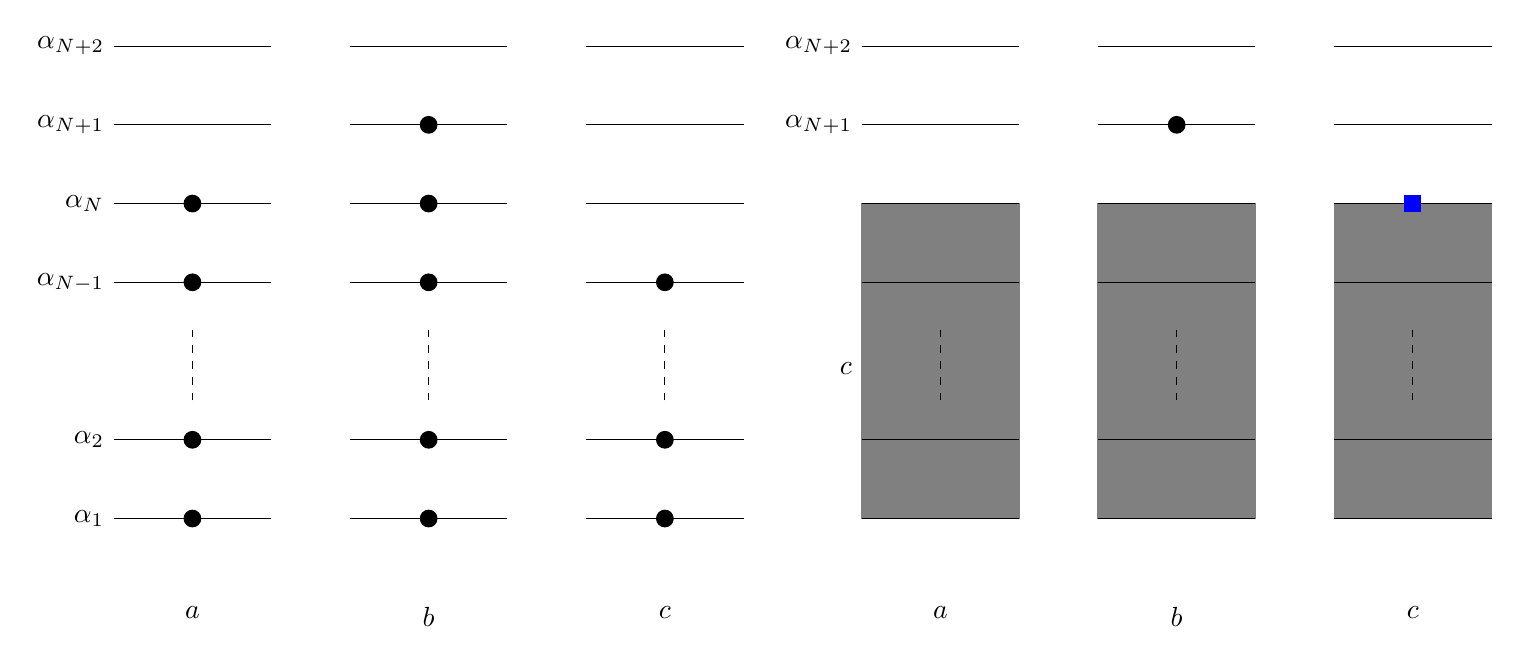
\begin{tikzpicture}
\draw (1,-1) node[anchor=north] {$\ket{a}$} -- (1,-1);
\draw (0,0) node[anchor=east] {$\alpha_1$} -- (2,0);
\draw (0,1) node[anchor=east] {$\alpha_2$} -- (2,1);
\draw (1,1.5) -- (1,1.6);
\draw (1,1.7) -- (1,1.8);
\draw (1,1.9) -- (1,2);
\draw (1,2.1) -- (1,2.2);
\draw (1,2.3) -- (1,2.4);
\draw (0,3) node[anchor=east] {$\alpha_{N-1}$} -- (2,3);
\draw (0,4) node[anchor=east] {$\alpha_N$}-- (2,4);
\draw (0,5) node[anchor=east] {$\alpha_{N+1}$}-- (2,5);
\draw (0,6) node[anchor=east] {$\alpha_{N+2}$} -- (2,6);
\filldraw [black] (1,0) circle (3pt);
\filldraw [black] (1,1) circle (3pt);
\filldraw [black] (1,3) circle (3pt);
\filldraw [black] (1,4) circle (3pt);

\draw (4,-1) node[anchor=north] {$\ket{b}$} -- (4,-1);
\draw (3,0) -- (5,0);
\draw (3,1) -- (5,1);
\draw (4,1.5) -- (4,1.6);
\draw (4,1.7) -- (4,1.8);
\draw (4,1.9) -- (4,2);
\draw (4,2.1) -- (4,2.2);
\draw (4,2.3) -- (4,2.4);
\draw (3,3) -- (5,3);
\draw (3,4) -- (5,4);
\draw (3,5) -- (5,5);
\draw (3,6) -- (5,6);
\filldraw [black] (4,0) circle (3pt);
\filldraw [black] (4,1) circle (3pt);
\filldraw [black] (4,3) circle (3pt);
\filldraw [black] (4,4) circle (3pt);
\filldraw [black] (4,5) circle (3pt);

\draw (7,-1) node[anchor=north] {$\ket{c}$} -- (7,-1);
\draw (6,0) -- (8,0);
\draw (6,1) -- (8,1);
\draw (7,1.5) -- (7,1.6);
\draw (7,1.7) -- (7,1.8);
\draw (7,1.9) -- (7,2);
\draw (7,2.1) -- (7,2.2);
\draw (7,2.3) -- (7,2.4);
\draw (6,3) -- (8,3);
\draw (6,4) -- (8,4);
\draw (6,5) -- (8,5);
\draw (6,6) -- (8,6);
\filldraw [black] (7,0) circle (3pt);
\filldraw [black] (7,1) circle (3pt);
\filldraw [black] (7,3) circle (3pt);

\draw (10.5,-1) node[anchor=north] {$\ket{a}$} -- (10.5,-1);
\filldraw [gray] (9.5,0) rectangle (11.5,4);
\draw (9.5,0) -- (11.5,0);
\draw (9.5,1) -- (11.5,1);
\draw (10.5,1.5) -- (10.5,1.6);
\draw (10.5,1.7) -- (10.5,1.8);
\draw (10.5,1.9) node[anchor=east] {$\ket{c}\hspace{1cm}$} -- (10.5,2);
\draw (10.5,2.1) -- (10.5,2.2);
\draw (10.5,2.3) -- (10.5,2.4);
\draw (9.5,3)  -- (11.5,3);
\draw (9.5,4)  -- (11.5,4);
\draw (9.5,5) node[anchor=east] {$\alpha_{{N+1}}$} -- (11.5,5);
\draw (9.5,6) node[anchor=east] {$\alpha_{N+2}$} -- (11.5,6);

\draw (13.5,-1) node[anchor=north] {$\ket{b}$} -- (13.5,-1);
\filldraw [gray] (12.5,0) rectangle (14.5,4);
\draw (12.5,0) -- (14.5,0);
\draw (12.5,1) -- (14.5,1);
\draw (13.5,1.5) -- (13.5,1.6);
\draw (13.5,1.7) -- (13.5,1.8);
\draw (13.5,1.9) -- (13.5,2);
\draw (13.5,2.1) -- (13.5,2.2);
\draw (13.5,2.3) -- (13.5,2.4);
\draw (12.5,3) -- (14.5,3);
\draw (12.5,4) -- (14.5,4);
\draw (12.5,5) -- (14.5,5);
\draw (12.5,6) -- (14.5,6);
\filldraw [black] (13.5,5) circle (3pt);

\draw (16.5,-1) node[anchor=north] {$\ket{c}$} -- (16.5,-1);
\filldraw [gray] (15.5,0) rectangle (17.5,4);
\draw (15.5,0) -- (17.5,0);
\draw (15.5,1) -- (17.5,1);
\draw (16.5,1.5) -- (16.5,1.6);
\draw (16.5,1.7) -- (16.5,1.8);
\draw (16.5,1.9) -- (16.5,2);
\draw (16.5,2.1) -- (16.5,2.2);
\draw (16.5,2.3) -- (16.5,2.4);
\draw (15.5,3) -- (17.5,3);
\draw (15.5,4) -- (17.5,4);
\draw (15.5,5) -- (17.5,5);
\draw (15.5,6) -- (17.5,6);
\filldraw [blue] (16.4, 3.9) rectangle (16.6,4.1) ;
\end{tikzpicture}}
\end{center}
\label{fig: Particle-hole figure}
\caption{Particle-Hole.}
\end{figure}

In the same way as we can construct a general slater determinant by letting the ordinary creation operators act on the vacuum state, we are now in a position to construct many-quasiparticle states by letting quasi-particle creation operators act on the reference state $\ket{r}$.
\begin{align}
\ket{ijkl..abcd..}_r \equiv \crequasi{i}\crequasi{j}\crequasi{k}\crequasi{l}..\crequasi{a}\crequasi{b}\crequasi{c}\crequasi{d}..\ket{r}.
\end{align}



\section{Normal-ordered Hamiltonian}

\subsection{Antisymmetrized wavefunction}
    \begin{align*}
        \Phi_{AS}(\alpha_1, \dots, \alpha_A; \mathbf{x}_1, \dots \mathbf{x}_A) &= 
            \frac{1}{\sqrt{A}} \sum_{\hat{P}} (-1)^P \hat{P} \prod_{i=1}^A \psi_{\alpha_i}(\mathbf{x}_i) \\
        &\equiv \ket{\alpha_1 \dots \alpha_A} \\
        &= a_{\alpha_1}^\dagger \dots a_{\alpha_A}^\dagger \ket{0}
    \end{align*}
    \begin{align*}
        a_p^\dagger\ket{0} = \ket{p}, \quad a_p \ket{q} = \delta_{pq}\ket{0}
    \end{align*}
    \begin{align*}
        \delta_{pq} &= \left\{a_p, a_q^\dagger \right\} \\
        0 = \left\{a_p^\dagger, a_q \right\} &= \left\{a_p, a_q \right\} = \left\{a_p^\dagger, a_q^\dagger \right\}
    \end{align*}
        \begin{equation*}
            \ket{\Phi_0} = \ket{\alpha_1 \dots \alpha_A}, \quad \alpha_1, \dots, \alpha_A \leq \alpha_F
        \end{equation*}
    \begin{align*}
        \left\{a_p^\dagger, a_q \right\}&= \delta_{pq}, p, q \leq \alpha_F & 
            \left\{a_p, a_q^\dagger \right\} &= \delta_{pq}, p, q > \alpha_F
    \end{align*}
        \begin{center}
        $i,j,\ldots \leq \alpha_F, \quad a,b,\ldots > \alpha_F, \quad p,q, \ldots - \textrm{any}$
        \end{center}
    \begin{align*}
        a_i\ket{\Phi_0} &= \ket{\Phi_i} & a_a^\dagger\ket{\Phi_0} &= \ket{\Phi^a} \\
        a_i^\dagger\ket{\Phi_0} &= 0 & a_a\ket{\Phi_0} &= 0
    \end{align*}
\subsection{Onebody and twobody operators}
        \begin{equation*}
            \hat{F} = \sum_{pq} \element{p}{\hat{f}}{q} a_p^\dagger a_q
        \end{equation*}
        \begin{align*}
            \hat{V} &= \frac{1}{4} \sum_{pqrs} \element{pq}{\hat{v}}{rs}_{AS} a_p^\dagger a_q^\dagger a_s a_r
            \equiv \frac{1}{4} \sum_{pqrs} \element{pq}{\hat{v}}{rs} a_p^\dagger a_q^\dagger a_s a_r \\
        \end{align*}
        where we have defined the antisymmetric matrix elements
        \begin{align*}
            \element{pq}{\hat{v}}{rs}_{AS} &= \element{pq}{\hat{v}}{rs} - \element{pq}{\hat{v}}{sr}.
        \end{align*}
        \begin{align*}
            \hat{V_3} &= \frac{1}{36} \sum_{pqrstu} \element{pqr}{\hat{v}_3}{stu}_{AS} 
                a_p^\dagger a_q^\dagger a_r^\dagger a_u a_t a_s
            \equiv \frac{1}{36} \sum_{pqrstu} \element{pqr}{\hat{v}_3}{stu}
                a_p^\dagger a_q^\dagger a_r^\dagger a_u a_t a_s
        \end{align*}
        \normalsize
        where we have defined the antisymmetric matrix elements
        \begin{align*}
            \element{pqr}{\hat{v}_3}{stu}_{AS} &= \element{pqr}{\hat{v}_3}{stu} + \element{pqr}{\hat{v}_3}{tus} + \element{pqr}{\hat{v}_3}{ust} \\
            & - \element{pqr}{\hat{v}_3}{sut} - \element{pqr}{\hat{v}_3}{tsu} - \element{pqr}{\hat{v}_3}{uts}.
        \end{align*}
        \begin{equation*}
            \left\{a_a a_b \ldots a_c^\dagger a_d^\dagger\right\} = 
                (-1)^P a_c^\dagger a_d^\dagger \ldots a_a a_b
        \end{equation*}
    All creation operators to the left and all annihilation operators to the right times a factor determined by how many operators have been switched.


    \subsection{The basics, Normal ordered Hamiltonian}
    The normal ordered Hamiltonian is given by
    \begin{align*}
        \hat{H}_N &= 
            \frac{1}{36} \sum_{\substack{
                        pqr \\
                        stu}}
                 \element{pqr}{\hat{v}_3}{stu} 
                    \normord{a^\dagger_p a^\dagger_q a^\dagger_r a_u a_t a_s} \nn
        & \quad + 
            \frac{1}{4} \sum_{pqrs} \bra{pq}\ket{rs} \normord{a^\dagger_p a^\dagger_q a_s  a_r} 
            + \sum_{pq} f_q^p \normord{a^\dagger_p a_q} \\
        &= \hat{H}_3^N + \hat{V}_N + \hat{F}_N
    \end{align*}
    where
    \begin{subequations}
    \begin{align*}
        \hat{F}_N &= \sum_{pq} f_q^p \normord{a^\dagger_p a_q} &
        \hat{V}_N &= \frac{1}{4} \sum_{pqrs} \bra{pq}\ket{rs} \normord{a^\dagger_p a^\dagger_q a_s  a_r} \\
        && \hat{H}_3^N &= 
                \frac{1}{36} \sum_{\substack{
                            pqr \\
                            stu}}
                     \element{pqr}{\hat{v}_3}{stu} 
                        \normord{a^\dagger_p a^\dagger_q a^\dagger_r a_u a_t a_s}
    \end{align*}
    \end{subequations}
    The amplitudes are given by
    \begin{subequations}
    \begin{align*}
        f_q^p &= \element{p}{\hat{h}_0}{q} + \sum_i \element{pi}{\hat{v}}{qi} 
            + \frac{1}{2} \sum_{ij} \element{pij}{\hat{v}_3}{qij} \\
        \bra{pq}\ket{rs} &= \element{pq}{\hat{v}}{rs} + \sum_i \element{pqi}{\hat{v}_3}{rsi},
    \end{align*}
    \end{subequations}
    In relation to the Hamiltonian, $\hat{H}_N$ is given by
    \begin{align*}
        \hat{H}_N &= \hat{H} - E_0 \\
        E_0 &= \element{\Phi_0}{\hat{H}}{\Phi_0} \\
            &= \sum_i \element{i}{\hat{h}_0}{i}
                + \frac{1}{2} \sum_{ij} \element{ij}{\hat{v}}{ij}
                + \frac{1}{6} \sum_{ijk} \element{ijk}{\hat{v}_3}{ijk},
    \end{align*}
    where $E_0$ is the energy expectation value between reference states.
    We start with the Hamiltonian
    \begin{equation*}
        \hat{H} = \hat{H}_1 + \hat{H}_2 + \hat{H}_3
    \end{equation*}
    where
    \begin{subequations}
        \begin{align*}
        \hat{H}_1 &= \sum_{pq} \element{p}{\hat{h}_0}{q} a^\dagger_p a_q \\
        \hat{H}_2 &= \frac{1}{4} \sum_{pqrs} \element{pq}{\hat{v}}{rs} a^\dagger_p a^\dagger_q a_s  a_r \\
        \hat{H}_3 &= \frac{1}{36} \sum_{\substack{
                            pqr \\
                            stu}}
                     \element{pqr}{\hat{v}_3}{stu} a^\dagger_p a^\dagger_q a^\dagger_r a_u a_t a_s
        \end{align*}
    \end{subequations}
    \begin{equation*}
        \hat{H}_1 = \sum_{pq} \element{p}{\hat{h}_0}{q} a^\dagger_p a_q
    \end{equation*}

    \begin{align*}
        a^\dagger_p a_q &= \left\{a^\dagger_p a_q\right\} + \left\{ 
    \contraction{}{a}{{}^{\dagger}_p}{a}
    a^\dagger_p a_q
    \right\} \nn
        &= \left\{a^\dagger_p a_q\right\} + \delta_{pq\in i}
    \end{align*}
    \begin{align*}
        \hat{H}_1 &= \sum_{pq} \element{p}{\hat{h}_0}{q} a^\dagger_p a_q \nn
            &= \sum_{pq} \element{p}{\hat{h}_0}{q} \left\{a^\dagger_p a_q\right\} + 
                \delta_{pq\in i} \sum_{pq} \element{p}{\hat{h}_0}{q} \nn
            &= \sum_{pq} \element{p}{\hat{h}_0}{q} \left\{a^\dagger_p a_q\right\} +
                \sum_i \element{i}{\hat{h}_0}{i}
    \end{align*}
    A onebody part
    \begin{equation*}
            \hat{F}_N \Leftarrow \sum_{pq} \element{p}{\hat{h}_0}{q} \left\{a^\dagger_p a_q\right\}
    \end{equation*}
    and a scalar part
    \begin{equation*}
                E_0 \Leftarrow \sum_i \element{i}{\hat{h}_0}{i}
    \end{equation*}
    \begin{equation*}
        \hat{H}_2 = \frac{1}{4} \sum_{pqrs} \element{pq}{\hat{v}}{rs} a^\dagger_p a^\dagger_q a_s  a_r
    \end{equation*}

\begin{align*}
    a^\dagger_p a^\dagger_q a_s  a_r &= \pause
        \normord{a^\dagger_p a^\dagger_q a_s  a_r} \nn
        & \quad + \normord{
            \contraction{a^\dagger_p}{a}{{}^\dagger_q}{a}
            a^\dagger_p a^\dagger_q a_s  a_r}
        + \normord{
            \contraction{a^\dagger_p}{a}{{}^\dagger_q a_s}{a}
            a^\dagger_p a^\dagger_q a_s  a_r}
        + \normord{
            \contraction{}{a}{{}^\dagger_p a^\dagger_q}{a}
            a^\dagger_p a^\dagger_q a_s  a_r} \nn
        & \quad + \normord{
            \contraction{}{a}{{}^\dagger_p a^\dagger_q a_s}{a}
            a^\dagger_p a^\dagger_q a_s  a_r}
        + \normord{
            \contraction[1.5ex]{}{a}{{}^\dagger_p a_q^\dagger a_s}{a}
            \contraction{a^\dagger_p}{a}{{}^\dagger_q}{a}
            a^\dagger_p a^\dagger_q a_s  a_r}
        + \normord{
            \contraction{}{a}{{}^\dagger_p a_q^\dagger}{a}
            \contraction[1.5ex]{a^\dagger_p}{a}{{}^\dagger_q a_s}{a}
            a^\dagger_p a^\dagger_q a_s  a_r} \nn
    &= \normord{a^\dagger_p a^\dagger_q a_s  a_r} \nn
        & \quad + \delta_{qs\in i} \normord{ a^\dagger_p a_r}
        - \delta_{qr \in i} \normord{a^\dagger_p a_s}
        - \delta_{ps \in i} \normord{a^\dagger_q a_r} \nn
        & \quad + \delta_{pr \in i} \normord{a^\dagger_q a_s} 
        + \delta_{pr \in i} \delta_{qs \in i} - \delta_{ps \in i} \delta_{qr \in i}
\end{align*}
    \begin{align*}
    \hat{H}_2 &= \frac{1}{4} \sum_{pqrs} \element{pq}{\hat{v}}{rs} a^\dagger_p a^\dagger_q a_s  a_r \nn
        &= \frac{1}{4} \sum_{pqrs} \element{pq}{\hat{v}}{rs} \normord{a^\dagger_p a^\dagger_q a_s  a_r} 
        + \quad \frac{1}{4} \sum_{pqrs} \Bigl( 
            \delta_{qs\in i} \element{pq}{\hat{v}}{rs} \normord{ a^\dagger_p a_r} \nn
        & \quad - \delta_{qr \in i} \element{pq}{\hat{v}}{rs} \normord{a^\dagger_p a_s}
            - \delta_{ps \in i}\element{pq}{\hat{v}}{rs} \normord{a^\dagger_q a_r} \nn
        & \quad + \delta_{pr \in i} \element{pq}{\hat{v}}{rs} \normord{a^\dagger_q a_s}
            + \delta_{pr \in i} \delta_{qs \in i}
            - \delta_{ps \in i} \delta_{qr \in i} \Bigr) \nn
    \end{align*}
    \begin{align*}
        &= \frac{1}{4} \sum_{pqrs} \element{pq}{\hat{v}}{rs} \normord{a^\dagger_p a^\dagger_q a_s  a_r} \nn
        & \quad + \frac{1}{4} \sum_{pqi} \Bigl(
            \element{pi}{\hat{v}}{qi} - \element{pi}{\hat{v}}{iq} - \element{ip}{\hat{v}}{qi} + \element{ip}{\hat{v}}{iq}
        \Bigr) \normord{a^\dagger_p a_q} \nn
        & \quad + \frac{1}{4} \sum_{ij} \Bigl( 
            \element{ij}{\hat{v}}{ij}
            - \element{ij}{\hat{v}}{ji}
        \Bigr) \nn
        &= \frac{1}{4} \sum_{pqrs} \element{pq}{\hat{v}}{rs} \normord{a^\dagger_p a^\dagger_q a_s  a_r}
            + \sum_{pqi} \element{pi}{\hat{v}}{qi} \normord{a^\dagger_p a_q} 
            + \frac{1}{2} \sum_{ij} \element{ij}{\hat{v}}{ij}
    \end{align*}
    A twobody part
    \begin{equation*}
            \hat{V}_N \Leftarrow \frac{1}{4} \sum_{pqrs} \element{pq}{\hat{v}}{rs} 
                \normord{a^\dagger_p a^\dagger_q a_s  a_r}
    \end{equation*}
    A onebody part
    \begin{equation*}
            \hat{F}_N \Leftarrow \sum_{pqi} \element{pi}{\hat{v}}{qi} \normord{a^\dagger_p a_q}
    \end{equation*}
    and a scalar part
    \begin{equation*}
                E_0 \Leftarrow \frac{1}{2} \sum_{ij} \element{ij}{\hat{v}}{ij}
    \end{equation*}
     Derive the normal-ordered form of the threebody part of the Hamiltonian.
    \begin{align*}
    \hat{H}_3 &= \frac{1}{36} \sum_{\substack{
                        pqr \\
                        stu}}
                 \element{pqr}{\hat{v}_3}{stu} a^\dagger_p a^\dagger_q a^\dagger_r a_u a_t a_s \\
        &= ?
    \end{align*}
    and specify the contributions to the twobody, onebody and the scalar part.
    \begin{align*}
        \hat{H}_N &= 
            \frac{1}{4} \sum_{pqrs} \bra{pq}\ket{rs} \normord{a^\dagger_p a^\dagger_q a_s  a_r} 
            + \sum_{pq} f_q^p \normord{a^\dagger_p a_q} \\
        &= \hat{V}_N + \hat{F}_N
    \end{align*}
    where
    \begin{subequations}
    \begin{align*}
        \hat{F}_N &= \sum_{pq} f_q^p \normord{a^\dagger_p a_q} \\
        \hat{V}_N &= \frac{1}{4} \sum_{pqrs} \bra{pq}\ket{rs} \normord{a^\dagger_p a^\dagger_q a_s  a_r} \\
    \end{align*}
    \end{subequations}
    The amplitudes are given by
    \begin{subequations}
    \begin{align*}
        f_q^p &= \element{p}{\hat{h}_0}{q} + \sum_i \element{pi}{\hat{v}}{qi} \\
        \bra{pq}\ket{rs} &= \element{pq}{\hat{v}}{rs}
    \end{align*}
    \end{subequations}
    In relation to the Hamiltonian, $\hat{H}_N$ is given by
    \begin{align*}
        \hat{H}_N &= \hat{H} - E_0 \\
        E_0 &= \element{\Phi_0}{\hat{H}}{\Phi_0} \\
            &= \sum_i \element{i}{\hat{h}_0}{i}
                + \frac{1}{2} \sum_{ij} \element{ij}{\hat{v}}{ij}
    \end{align*}
    where $E_0$ is the energy expectation value between reference states.




\section{Diagrams}
Although Wick's theorem adds considerable simplifications to the calculation of various expectation values, the human brain is, sadly, not well suited for finding complicated combinations of
contractions using Wick's theorem.
As an example, we present a string of operators
arising from the evaluation of the transition probability from a 1p-1h excitation
to another 1p-1h excitation for the two-body potential, 
\begin{equation}
\label{eq:manybody:example}
\langle \Phi_i^a | \hat{V} | \Phi_j^b \rangle
\rightarrow
\hat{i}^{\dagger} \hat{a} \hspace{2mm} \hat{p}^{\dagger} \hat{q}^{\dagger}
\hat{s} \hat{r} \hspace{2mm} \hat{b}^{\dagger} \hat{j} .
\end{equation}
Although this expression only contains eight operators, it leads to fourteen nonzero,
fully contracted, terms.
One needs to be focused and systematic in order to calculate all terms correctly.
However, the brain seems to be good at visualizing mental images, and therefore a
graphical presentation of the formulas could serve us well.


The graphical approach presented here originated in quantum field theory,
developed by Richard Feynman~\cite{RevModPhys.20.367,PhysRev.76.769}.
Although originally meant to be used on time dependent transitions from one
state to another, it is presented here without a time ordering (following~\cite{shavitt2009many}).
It does, however, restrict the order in which operators are applied.

Diagrams start out with the reference ket state, denoted by two horizontal lines at
the bottom, and end out with the reference bra state, as two horizontal lines
at the top. 
Particle operators are lines pointing upwards, whereas holes point downwards.
In this fashion, determinants with excitations from the reference state can be visualized as
\begin{eqnarray}
\langle \Phi_i^a | = \langle \Phi | \hat{i}^{\dagger}\hat{a} =& 
\parbox{30mm}{
    \textrm{
    \begin{fmffile}{fmf-oneponehbra}
        \begin{fmfgraph*}(50,50)
            \fmfbottom{i1,i2} \fmftop{o1,o2}
            \fmf{phantom}{i1,hb,pb,i2}
            \fmf{double}{o1,ht,pt,o2}
            \fmffreeze
            \fmf{electron,label=$i$}{ht,hb}
            \fmf{electron,label=$a$}{pb,pt}
        \end{fmfgraph*}
    \end{fmffile}
    }
} \\
|\Phi_{ij}^{ab} \rangle = \hat{a}^{\dagger}\hat{b}^{\dagger}\hat{j}\hat{i}|\Phi \rangle =& 
\parbox{40mm}{
    \textrm{
    \begin{fmffile}{fmf-twoptwohket}
        \begin{fmfgraph*}(100,50)
            \fmfbottom{i1,i2} \fmftop{o1,o2}
            \fmf{double}{i1,h1b,p1b,dummyb,h2b,p2b,i2}
            \fmf{phantom}{o1,h1t,p1t,dummyt,h2t,p2t,o2}
            \fmffreeze
            \fmf{electron,label=$i$}{h1t,h1b}
            \fmf{electron,label=$a$}{p1b,p1t}
            \fmf{electron,label=$j$}{h2t,h2b}
            \fmf{electron,label=$b$}{p2b,p2t}
        \end{fmfgraph*}
    \end{fmffile}
    }
} .
\end{eqnarray}


One-body operators are presented as two electron lines connected to a dashed line with a cross,
\begin{equation}
\hat{H^{(0)}} = \sum_{pq} \langle p | \hat{h^{(0)}} | \hat{q} \rangle \hat{p}^{\dagger}\hat{q} =
\parbox{30mm}{
	\textrm{
	\begin{fmffile}{fmf-onebodyoperator}
		\begin{fmfgraph*}(50,50)
			\fmfbottom{i1,i2} \fmftop{o1,o2}
			\fmf{electron,label=$q$}{i1,f1}
			\fmf{electron,label=$p$}{f1,o1}
			\fmf{dashes}{f1,f2}
			\fmfv{decor.shape=cross}{f2}
			\fmf{phantom}{i2,f2}
			\fmf{phantom}{f2,o2}
		\end{fmfgraph*}
	\end{fmffile}
	}
}
\end{equation}
Two-body operators are represented similarly, but have two incoming and two outgoing lines due to the two-body nature,
\begin{equation}
\hat{H}^{(1)} = \frac{1}{4}\sum_{pqrs} \langle pq | | rs \rangle \hat{p}^{\dagger}\hat{q}^{\dagger} \hat{s} \hat{r} =
\parbox{30mm}{
	\textrm{
	\begin{fmffile}{fmf-twobodyoperator}
		\begin{fmfgraph*}(50,50)
			\fmfbottom{i1,i2} \fmftop{o1,o2}
			\fmf{electron,label=$r$}{i1,f1}
			\fmf{electron,label=$p$}{f1,o1}
			\fmf{dashes}{f1,f2}
			\fmf{electron,label=$s$}{i2,f2}
			\fmf{electron,label=$q$}{f2,o2}
		\end{fmfgraph*}
	\end{fmffile}
	}
} .
\end{equation}


The idea now is to represent contractions by connecting lines, and because only fully contracted terms are nonzero within the reference state, all lines should be connected.
All \textit{free} indexes are meant to be summed over, and the matrix elements are found by replacing $q$ with the label of incoming line and $p$ with the outgoing label in the one-body case.
In the two-body case we replace $r/s$ with left/right incoming line and $p/q$ with left/right outgoing line.
To determine the correct phase factor, one needs to count the number of hole lines and the number of closed paths.
When counting the number of closed paths we will consider associated particle-hole pairs as if they were connected in the reference states.
The phase factor will in the end be $(-1)^{l + h}$, where $l$ is the number of closed paths (loops) and $h$ is the number of hole lines.


To illustrate the use of diagrams, we return to the example in the introduction, eq.~\eqref{eq:manybody:example}.
This expression is evaluated to four unique ways of connecting the diagrams;

\begin{equation}
\label{eq:manybody:iavbjDiag}
\begin{split}
\langle \Phi_i^a | \hat{V} | \Phi_j^b \rangle
&= 
\overbrace{
\parbox{35mm}{
	\textrm{
	\begin{fmffile}{fmf-example-term1}
		\begin{fmfgraph*}(80,80) \fmfkeep{fmf-example-term1}
			\fmfbottom{i1,i2} \fmftop{o1,o2}
			%Reference states
			\fmf{double}{i1,b1,dummy1,b2,i2}
			\fmf{double}{o1,t1,dummy2,t2,o2}
			\fmffreeze
			%Operator line
			\fmf{dashes}{g1,g2}
			%Electrons		
			\fmf{electron,label=$j$}{g1,b1}
			\fmf{electron,label=$b$}{b2,g2}
			\fmf{electron,label=$i$}{t1,g1}
			\fmf{electron,label=$a$}{g2,t2}
		\end{fmfgraph*}
	\end{fmffile}
	}
}
}^{(a)}
+
\overbrace{
\parbox{35mm}{
	\textrm{
	\begin{fmffile}{fmf-example-term2}
		\begin{fmfgraph*}(80,80) \fmfkeep{fmf-example-term2}
			\fmfbottom{i1,i2} \fmftop{o1,o2}
			%Reference states
			\fmf{double}{i1,b1,dummy1,b2,i2}
			\fmf{double}{o1,t1,dummy2,t2,o2}
			\fmffreeze
			%Operator line
			\fmf{dashes}{g1,g2}
			\fmf{phantom}{b1,loop}
			\fmf{phantom}{t1,loop}
			%Electrons		
			\fmf{electron,label=$b$}{b2,g2}
			\fmf{electron,label=$a$}{g2,t2}
			\fmf{electron,label=$i$}{t1,holeconnect}
			\fmf{electron,label=$j$}{holeconnect,b1}
			%Electron hole loop
			\fmf{electron,right,tension=0.3,label=$k$}{g1,loop}
			\fmf{electron,right,tension=0.3}{loop,g1}
		\end{fmfgraph*}
	\end{fmffile}
	}
}
}^{(b)} \\
&+
\underbrace{
\parbox{35mm}{
	\textrm{
	\begin{fmffile}{fmf-example-term3}
		\begin{fmfgraph*}(80,80) \fmfkeep{fmf-example-term3}
			\fmfbottom{i1,i2} \fmftop{o1,o2}
			%Reference states
			\fmf{double}{i1,b1,dummy1,b2,i2}
			\fmf{double}{o1,t1,dummy2,t2,o2}
			\fmffreeze
			%Operator line
			\fmf{dashes}{g1,g2}
			\fmf{phantom}{b2,loop}
			\fmf{phantom}{t2,loop}
			%Electrons		
			\fmf{electron,label=$b$}{b2,partconnect}
			\fmf{electron,label=$a$}{partconnect,t2}
			\fmf{electron,label=$i$}{t1,g1}
			\fmf{electron,label=$j$}{g1,b1}
			%Electron hole loop
			\fmf{electron,left,tension=0.3}{g2,loop}
			\fmf{electron,left,tension=0.3,label=$k$}{loop,g2}
		\end{fmfgraph*}
	\end{fmffile}
	}
}
}_{(c)}
+
\underbrace{
\parbox{35mm}{
	\textrm{
	\begin{fmffile}{fmf-example-term4}
		\begin{fmfgraph*}(80,80) \fmfkeep{fmf-example-term4}
			\fmfbottom{i1,i2} \fmftop{o1,o2}
			%Reference states
			\fmf{double}{i1,b1,b2,b3,b4,b5,i2}
			\fmf{double}{o1,t1,t2,t3,t4,t5,o2}
			\fmffreeze
			%Connecting points for hole loops
			\fmf{phantom}{b3,loop1,t3}
			\fmf{phantom}{i2,loop2,o2}
			\fmffreeze
			%Operator
			\fmf{dashes}{g1,g2}
			%Hole loops
			\fmf{electron,right,label=$k$,tension=0.3}{g1,loop1}
			\fmf{electron,right,tension=0.3}{loop1,g1}
			\fmf{electron,left,label=$l$,tension=0.3}{g2,loop2}
			\fmf{electron,left,tension=0.3}{loop2,g2}
			%Electronlines
			\fmf{electron,label=$i$}{t1,holeconnect}
			\fmf{electron,label=$j$}{holeconnect,b1}
			\fmf{electron,label=$b$}{b2,partconnect}
			\fmf{electron,label=$a$}{partconnect,t2}
		\end{fmfgraph*}
	\end{fmffile}
	}
} 
}_{(d)}
.
\end{split}
\end{equation}
\begin{enumerate}[{\bf Term (\ref{eq:manybody:iavbjDiag}a)}]
\item has no free indexes since all lines are connected to the particle and hole indices already defined in the reference states.
The corresponding matrix element is $\langle ja || ib \rangle$.
Having two hole lines, one closed loop, and in total four equal terms, 
\begin{equation}
\parbox{23mm}{
	\textrm{
	\begin{fmffile}{fmf-example-term1-1}
		\begin{fmfgraph*}(50,50)
			\fmfbottom{i1,i2} \fmftop{o1,o2}
			%Reference states
			\fmf{double}{i1,b1,dummy1,b2,i2}
			\fmf{double}{o1,t1,dummy2,t2,o2}
			\fmffreeze
			%Operator line
			\fmf{dashes}{g1,g2}
			%Electrons		
			\fmf{electron}{g1,b1}
			\fmf{electron}{b2,g2}
			\fmf{electron}{t1,g1}
			\fmf{electron}{g2,t2}
		\end{fmfgraph*}
	\end{fmffile}
	}
}
=
\parbox{23mm}{
	\textrm{
	\begin{fmffile}{fmf-example-term1-2}
		\begin{fmfgraph*}(50,50) \fmfkeep{fmf-example-term1-2}
			\fmfbottom{i1,i2} \fmftop{o1,o2}
			%Reference states
			\fmf{double}{i1,b1,dummy1,b2,i2}
			\fmf{double}{o1,t1,dummy2,t2,o2}
			\fmffreeze
			%Operator line
			\fmf{dashes}{g1,g2}
			\fmf{phantom}{g1,b1}
			\fmf{phantom}{b2,g2}
			\fmf{phantom}{t1,g1}
			\fmf{phantom}{g2,t2}			
			\fmffreeze
			%Electrons		
			\fmf{electron}{g2,b1}
			\fmf{electron}{b2,g1}
			\fmf{electron}{t1,g2}
			\fmf{electron}{g1,t2}
		\end{fmfgraph*}
	\end{fmffile}
	}
}
=
\parbox{23mm}{
	\textrm{
	\begin{fmffile}{fmf-example-term1-3}
		\begin{fmfgraph*}(50,50) \fmfkeep{fmf-example-term1-3}
			\fmfbottom{i1,i2} \fmftop{o1,o2}
			%Reference states
			\fmf{double}{i1,b1,dummy1,b2,i2}
			\fmf{double}{o1,t1,dummy2,t2,o2}
			\fmffreeze
			%Operator line
			\fmf{dashes}{g1,g2}
			\fmf{phantom}{g1,b1}
			\fmf{phantom}{b2,g2}
			\fmf{phantom}{t1,g1}
			\fmf{phantom}{g2,t2}			
			\fmffreeze
			%Electrons		
			\fmf{electron}{g1,b1}
			\fmf{electron}{b2,g1}
			\fmf{electron}{t1,g2}
			\fmf{electron}{g2,t2}
		\end{fmfgraph*}
	\end{fmffile}
	}
}
=
\parbox{23mm}{
	\textrm{
	\begin{fmffile}{fmf-example-term1-4}
		\begin{fmfgraph*}(50,50) \fmfkeep{fmf-example-term1-4}
			\fmfbottom{i1,i2} \fmftop{o1,o2}
			%Reference states
			\fmf{double}{i1,b1,dummy1,b2,i2}
			\fmf{double}{o1,t1,dummy2,t2,o2}
			\fmffreeze
			%Operator line
			\fmf{dashes}{g1,g2}
			\fmf{phantom}{g1,b1}
			\fmf{phantom}{b2,g2}
			\fmf{phantom}{t1,g1}
			\fmf{phantom}{g2,t2}			
			\fmffreeze
			%Electrons		
			\fmf{electron}{g2,b1}
			\fmf{electron}{b2,g2}
			\fmf{electron}{t1,g1}
			\fmf{electron}{g1,t2}
		\end{fmfgraph*}
	\end{fmffile}
	}
} ,
\end{equation}
the total factor in front should be $(-1)^{2+1} \cdot 4 \cdot \frac{1}{4} = -1$.
\item corresponds to the element $\delta_{ij} \langle ka || kb \rangle$, where the Kronecker delta function follows from the contracted hole lines between $i$ and $j$.
There are two hole lines, two loops, and in total four equal terms,
\begin{equation}
\parbox{23mm}{
	\textrm{
	\begin{fmffile}{fmf-example-term2-1}
		\begin{fmfgraph*}(50,50)
			\fmfbottom{i1,i2} \fmftop{o1,o2}
			%Reference states
			\fmf{double}{i1,b1,dummy1,b2,i2}
			\fmf{double}{o1,t1,dummy2,t2,o2}
			\fmffreeze
			%Operator line
			\fmf{dashes}{g1,g2}
			\fmf{phantom}{b1,loop}
			\fmf{phantom}{t1,loop}
			%Electrons		
			\fmf{electron}{b2,g2}
			\fmf{electron}{g2,t2}
			\fmf{electron}{t1,holeconnect}
			\fmf{electron}{holeconnect,b1}
			%Electron hole loop
			\fmf{electron,right,tension=0.3}{g1,loop}
			\fmf{electron,right,tension=0.3}{loop,g1}
		\end{fmfgraph*}
	\end{fmffile}
	}
}
=
\parbox{23mm}{
	\textrm{
	\begin{fmffile}{fmf-example-term2-2}
		\begin{fmfgraph*}(50,50)
			\fmfbottom{i1,i2} \fmftop{o1,o2}
			%Reference states
			\fmf{double}{i1,b1,dummy1,b2,i2}
			\fmf{double}{o1,t1,dummy2,t2,o2}
			\fmffreeze
			%Operator line
			\fmf{dashes}{g1,g2}
			\fmf{phantom}{b1,g1}
			\fmf{phantom}{t1,g1}
			\fmf{phantom}{g2,loop}
			\fmf{phantom}{i2,loop,o2}
			\fmffreeze
			%Electrons		
			\fmf{electron}{b2,g1}
			\fmf{electron}{g1,t2}
			\fmf{electron}{t1,holeconnect}
			\fmf{electron}{holeconnect,b1}
			%Electron hole loop
			\fmf{electron,right,tension=0.3}{g2,loop}
			\fmf{electron,right,tension=0.3}{loop,g2}
		\end{fmfgraph*}
	\end{fmffile}
	}
}
=
\parbox{23mm}{
	\textrm{
	\begin{fmffile}{fmf-example-term2-3}
		\begin{fmfgraph*}(50,50)
			\fmfbottom{i1,i2} \fmftop{o1,o2}
			%Reference states
			\fmf{double}{i1,b1,dummy1,b2,i2}
			\fmf{double}{o1,t1,dummy2,t2,o2}
			\fmffreeze
			%Operator line
			\fmf{dashes}{g1,gmiddle,g2}
			\fmf{phantom}{b1,g1}
			\fmf{phantom}{t1,g1}
			\fmf{phantom}{i2,g2,o2}
			\fmffreeze
			%Electrons		
			\fmf{electron}{b2,g2}
			\fmf{electron}{g1,t2}
			\fmf{electron}{t1,holeconnect}
			\fmf{electron}{holeconnect,b1}
			%Electron hole loop
			\fmf{electron,right,tension=0.5}{g2,gmiddle}
			\fmf{electron,left,tension=0.5}{gmiddle,g1}
		\end{fmfgraph*}
	\end{fmffile}
	}
}
=
\parbox{23mm}{
	\textrm{
	\begin{fmffile}{fmf-example-term2-4}
		\begin{fmfgraph*}(50,50)
			\fmfbottom{i1,i2} \fmftop{o1,o2}
			%Reference states
			\fmf{double}{i1,b1,dummy1,b2,i2}
			\fmf{double}{o1,t1,dummy2,t2,o2}
			\fmffreeze
			%Operator line
			\fmf{dashes}{g1,gmiddle,g2}
			\fmf{phantom}{b1,g1}
			\fmf{phantom}{t1,g1}
			\fmf{phantom}{i2,g2,o2}
			\fmffreeze
			%Electrons		
			\fmf{electron}{b2,g1}
			\fmf{electron}{g2,t2}
			\fmf{electron}{t1,holeconnect}
			\fmf{electron}{holeconnect,b1}
			%Electron hole loop
			\fmf{electron,left,tension=0.5}{g1,gmiddle}
			\fmf{electron,right,tension=0.5}{gmiddle,g2}
		\end{fmfgraph*}
	\end{fmffile}
	}
} .
\end{equation}
\item is similar to (\ref{eq:manybody:iavbjDiag}b), except how the Kronecker delta connects the particle lines $a$ and $b$ instead. There are now three hole lines, two loops and four  equal terms;
\begin{equation}
\parbox{23mm}{
	\textrm{
	\begin{fmffile}{fmf-example-term3-1}
		\begin{fmfgraph*}(50,50)
			\fmfbottom{i1,i2} \fmftop{o1,o2}
			%Reference states
			\fmf{double}{i1,b1,dummy1,b2,i2}
			\fmf{double}{o1,t1,dummy2,t2,o2}
			\fmffreeze
			%Operator line
			\fmf{dashes}{g1,g2}
			\fmf{phantom}{b2,loop}
			\fmf{phantom}{t2,loop}
			%Electrons		
			\fmf{electron}{b2,partconnect}
			\fmf{electron}{partconnect,t2}
			\fmf{electron}{t1,g1}
			\fmf{electron}{g1,b1}
			%Electron hole loop
			\fmf{electron,left,tension=0.3}{g2,loop}
			\fmf{electron,left,tension=0.3}{loop,g2}
		\end{fmfgraph*}
	\end{fmffile}
	}
}
=
\parbox{23mm}{
	\textrm{
	\begin{fmffile}{fmf-example-term3-2}
		\begin{fmfgraph*}(50,50)
			\fmfbottom{i1,i2} \fmftop{o1,o2}
			%Reference states
			\fmf{double}{i1,b1,dummy1,b2,i2}
			\fmf{double}{o1,t1,dummy2,t2,o2}
			\fmffreeze
			%Operator line
			\fmf{dashes}{g1,g2}
			\fmf{phantom}{b2,g2}
			\fmf{phantom}{t2,g2}
			\fmf{phantom}{g1,loop}
			\fmf{phantom}{i1,loop,o1}
			\fmffreeze
			%Electrons		
			\fmf{electron}{b2,partconnect}
			\fmf{electron}{partconnect,t2}
			\fmf{electron}{t1,g2}
			\fmf{electron}{g2,b1}
			%Electron hole loop
			\fmf{electron,left,tension=0.3}{g1,loop}
			\fmf{electron,left,tension=0.3}{loop,g1}			
		\end{fmfgraph*}
	\end{fmffile}
	}
}
=
\parbox{23mm}{
	\textrm{
	\begin{fmffile}{fmf-example-term3-3}
		\begin{fmfgraph*}(50,50)
			\fmfbottom{i1,i2} \fmftop{o1,o2}
			%Reference states
			\fmf{double}{i1,b1,dummy1,b2,i2}
			\fmf{double}{o1,t1,dummy2,t2,o2}
			\fmffreeze
			%Operator line
			\fmf{dashes}{g1,gmiddle,g2}
			\fmf{phantom}{i1,g1,o1}
			\fmf{phantom}{b2,g2,t2}
			\fmffreeze
			%Electrons		
			\fmf{electron}{b2,partconnect}
			\fmf{electron}{partconnect,t2}
			\fmf{electron}{t1,g2}
			\fmf{electron}{g1,b1}
			%Electron hole loop
			\fmf{electron,left,tension=0.5}{g2,gmiddle}
			\fmf{electron,right,tension=0.5}{gmiddle,g1}			
		\end{fmfgraph*}
	\end{fmffile}
	}
}
=
\parbox{23mm}{
	\textrm{
	\begin{fmffile}{fmf-example-term3-4}
		\begin{fmfgraph*}(50,50)
			\fmfbottom{i1,i2} \fmftop{o1,o2}
			%Reference states
			\fmf{double}{i1,b1,dummy1,b2,i2}
			\fmf{double}{o1,t1,dummy2,t2,o2}
			\fmffreeze
			%Operator line
			\fmf{dashes}{g1,gmiddle,g2}
			\fmf{phantom}{i1,g1,o1}
			\fmf{phantom}{b2,g2,t2}
			\fmffreeze
			%Electrons		
			\fmf{electron}{b2,partconnect}
			\fmf{electron}{partconnect,t2}
			\fmf{electron}{t1,g1}
			\fmf{electron}{g2,b1}
			%Electron hole loop
			\fmf{electron,right,tension=0.5}{g1,gmiddle}
			\fmf{electron,left,tension=0.5}{gmiddle,g2}			
		\end{fmfgraph*}
	\end{fmffile}
	}
} .
\end{equation}
\item has three hole lines, three loops, but only two equal diagrams can be created, namely
\begin{equation}
\parbox{23mm}{
	\textrm{
	\begin{fmffile}{fmf-example-term4-1}
		\begin{fmfgraph*}(50,50) 
			\fmfbottom{i1,i2} \fmftop{o1,o2}
			%Reference states
			\fmf{double}{i1,b1,b2,b3,b4,b5,i2}
			\fmf{double}{o1,t1,t2,t3,t4,t5,o2}
			\fmffreeze
			%Connecting points for hole loops
			\fmf{phantom}{b3,loop1,t3}
			\fmf{phantom}{i2,loop2,o2}
			\fmffreeze
			%Operator
			\fmf{dashes}{g1,g2}
			%Hole loops
			\fmf{electron,right,tension=0.3}{g1,loop1}
			\fmf{electron,right,tension=0.3}{loop1,g1}
			\fmf{electron,left,tension=0.3}{g2,loop2}
			\fmf{electron,left,tension=0.3}{loop2,g2}
			%Electronlines
			\fmf{electron}{t1,holeconnect}
			\fmf{electron}{holeconnect,b1}
			\fmf{electron}{b2,partconnect}
			\fmf{electron}{partconnect,t2}
		\end{fmfgraph*}
	\end{fmffile}
	}
}
=
\parbox{23mm}{
	\textrm{
	\begin{fmffile}{fmf-example-term4-2}
		\begin{fmfgraph*}(50,50) 
			\fmfbottom{i1,i2} \fmftop{o1,o2}
			%Reference states
			\fmf{double}{i1,b1,b2,b3,b4,i2}
			\fmf{double}{o1,t1,t2,t3,t4,o2}
			\fmffreeze
			%Operator
			\fmf{phantom}{i2,g2,o2}
			\fmffreeze
			\fmf{dashes}{g1,gmiddle,g2}
			\fmf{phantom}{b2,g1,t2}
			\fmffreeze
			%Hole loops
			\fmf{electron,left,tension=0.5}{g1,gmiddle}
			\fmf{electron,right,tension=0.5}{gmiddle,g2}
			\fmf{electron,right,tension=0.5}{g2,gmiddle}
			\fmf{electron,left,tension=0.5}{gmiddle,g1}
			%Electronlines
			\fmf{electron}{t1,holeconnect}
			\fmf{electron}{holeconnect,b1}
			\fmf{electron}{b2,partconnect}
			\fmf{electron}{partconnect,t2}
		\end{fmfgraph*}
	\end{fmffile}
	}
} .
\end{equation}
\end{enumerate}

We then have in total
\begin{equation}
\begin{split}
\langle \Phi_i^a | \hat{V} | \Phi_j^b \rangle
&=
\overbrace{(-1)^{1+2}\cdot 4 \cdot \frac{1}{4} \langle ja || ib \rangle}^{(a)}
+
\overbrace{(-1)^{2+2} \cdot 4 \cdot \frac{1}{4} \sum_k \delta_{ij} \langle ka || kb \rangle}^{(b)} \\
&+
\underbrace{(-1)^{2+3} \cdot 4 \cdot \frac{1}{4} \sum_k \delta_{ab} \langle jk || ik \rangle}_{(c)}
+
\underbrace{(-1)^{3+3} \cdot 2 \frac{1}{4} \sum_{kl} \delta_{ab} \delta_{ij} \langle kl || kl \rangle }_{(d)}\\
&=  - \langle ja || ib \rangle
+  \sum_k \delta_{ij} \langle ka || kb \rangle 
- \sum_k \delta_{ab} \langle jk || ik \rangle
+ \frac{1}{2} \sum_{kl} \delta_{ab} \delta_{ij} \langle kl || kl \rangle  .
\end{split}
\end{equation}
We will return to diagrams later.


\section{Bit operations and creation and annihilation operators}

In the build-up of a shell model code that is meant to tackle large dimensionalities
is the action of the Hamiltonian $\hat{H}$ on a 
Slater determinant represented in second quantization as
\[
\ket{\alpha_1\dots \alpha_n} = a_{\alpha_1}^\dagger a_{\alpha_2}^\dagger \dots a_{\alpha_n}^\dagger \ket{0}.
\]
The time consuming part stems from the action of the Hamiltonian
on the above determinant,
\[
\left(\sum_{\alpha\beta} \element{\alpha}{t+u}{\beta} a_\alpha^\dagger a_\beta + \frac{1}{4} \sum_{\alpha\beta\gamma\delta}
		\element{\alpha \beta}{V}{\gamma \delta} a_\alpha^\dagger a_\beta^\dagger a_\delta a_\gamma\right)a_{\alpha_1}^\dagger a_{\alpha_2}^\dagger \dots a_{\alpha_n}^\dagger \ket{0}.
\]
A practically useful way to implement this action is to encode a Slater determinant as a bit pattern. 

Assume that we have at our disposal $n$ different single-particle orbits
$\alpha_0,\alpha_2,\dots,\alpha_{n-1}$ and that we can distribute  among these orbits $N\le n$ particles.

A Slater  determinant can then be coded as an integer of $n$ bits. As an example, if we have $n=16$ single-particle states
$\alpha_0,\alpha_1,\dots,\alpha_{15}$ and $N=4$ fermions occupying the states $\alpha_3$, $\alpha_6$, $\alpha_{10}$ and $\alpha_{13}$
we could write this Slater determinant as  
\[
\Phi_{\Lambda} = a_{\alpha_3}^\dagger a_{\alpha_6}^\dagger a_{\alpha_{10}}^\dagger a_{\alpha_{13}}^\dagger \ket{0}.
\]
The unoccupied single-particle states have bit value $0$ while the occupied ones are represented by bit state $1$. 
In the binary notation we would write this   16 bits long integer as
\[
\begin{array}{cccccccccccccccc}
{\alpha_0}&{\alpha_1}&{\alpha_2}&{\alpha_3}&{\alpha_4}&{\alpha_5}&{\alpha_6}&{\alpha_7} & {\alpha_8} &{\alpha_9} & {\alpha_{10}} &{\alpha_{11}} &{\alpha_{12}} &{\alpha_{13}} &{\alpha_{14}} & {\alpha_{15}} \\
{0} & {0} &{0} &{1} &{0} &{0} &{1} &{0} &{0} &{0} &{1} &{0} &{0} &{1} &{0} & {0} \\
\end{array}
\]
which translates into the decimal number
\[
2^3+2^6+2^{10}+2^{13}=9288.
\]
We can thus encode a Slater determinant as a bit pattern.

With $N$ particles that can be distributed over $n$ single-particle states, the total number of Slater determinats (and defining thereby the dimensionality of the system) is
\[
\mathrm{dim}(\mathcal{H}) = \left(\begin{array}{c} n \\N\end{array}\right).
\]
The total number of bit patterns is $2^n$. 

We assume again that we have at our disposal $n$ different single-particle orbits
$\alpha_0,\alpha_2,\dots,\alpha_{n-1}$ and that we can distribute  among these orbits $N\le n$ particles.
The ordering among these states is important as it defines the order of the creation operators.
We will write the determinant 
\[
\Phi_{\Lambda} = a_{\alpha_3}^\dagger a_{\alpha_6}^\dagger a_{\alpha_{10}}^\dagger a_{\alpha_{13}}^\dagger \ket{0},
\]
in a more compact way as 
\[
\Phi_{3,6,10,13} = |0001001000100100\rangle.
\]
The action of a creation operator is thus
\[
a^\dagger_{\alpha_4}\Phi_{3,6,10,13} = a^\dagger_{\alpha_4}|0001001000100100\rangle=a^\dagger_{\alpha_4}a_{\alpha_3}^\dagger a_{\alpha_6}^\dagger a_{\alpha_{10}}^\dagger a_{\alpha_{13}}^\dagger \ket{0},
\]
which becomes
\[
-a_{\alpha_3}^\dagger a^\dagger_{\alpha_4} a_{\alpha_6}^\dagger a_{\alpha_{10}}^\dagger a_{\alpha_{13}}^\dagger \ket{0}=-|0001101000100100\rangle.
\]

Similarly
\[
a^\dagger_{\alpha_6}\Phi_{3,6,10,13} = a^\dagger_{\alpha_6}|0001001000100100\rangle=a^\dagger_{\alpha_6}a_{\alpha_3}^\dagger a_{\alpha_6}^\dagger a_{\alpha_{10}}^\dagger a_{\alpha_{13}}^\dagger \ket{0},
\]
which becomes
\[
-a^\dagger_{\alpha_4} (a_{\alpha_6}^\dagger)^ 2 a_{\alpha_{10}}^\dagger a_{\alpha_{13}}^\dagger \ket{0}=0!
\]
This gives a simple recipe:  
\begin{itemize}
\item If one of the bits $b_j$ is $1$ and we act with a creation operator on this bit, we return a null vector
\item  If $b_j=0$, we set it to $1$ and return a sign factor $(-1)^l$, where $l$ is the number of bits set before bit $j$.
\end{itemize}

Consider the action of $a^\dagger_{\alpha_2}$ on various slater determinants:
\[
\begin{array}{ccc}
a^\dagger_{\alpha_2}\Phi_{00111}& = a^\dagger_{\alpha_2}|00111\rangle&=0\times |00111\rangle\\
a^\dagger_{\alpha_2}\Phi_{01011}& = a^\dagger_{\alpha_2}|01011\rangle&=(-1)\times |01111\rangle\\
a^\dagger_{\alpha_2}\Phi_{01101}& = a^\dagger_{\alpha_2}|01101\rangle&=0\times |01101\rangle\\
a^\dagger_{\alpha_2}\Phi_{01110}& = a^\dagger_{\alpha_2}|01110\rangle&=0\times |01110\rangle\\
a^\dagger_{\alpha_2}\Phi_{10011}& = a^\dagger_{\alpha_2}|10011\rangle&=(-1)\times |10111\rangle\\
a^\dagger_{\alpha_2}\Phi_{10101}& = a^\dagger_{\alpha_2}|10101\rangle&=0\times |10101\rangle\\
a^\dagger_{\alpha_2}\Phi_{10110}& = a^\dagger_{\alpha_2}|10110\rangle&=0\times |10110\rangle\\
a^\dagger_{\alpha_2}\Phi_{11001}& = a^\dagger_{\alpha_2}|11001\rangle&=(+1)\times |11101\rangle\\
a^\dagger_{\alpha_2}\Phi_{11010}& = a^\dagger_{\alpha_2}|11010\rangle&=(+1)\times |11110\rangle\\
\end{array}
\]

We have an SD representation
\[
\Phi_{\Lambda} = a_{\alpha_0}^\dagger a_{\alpha_3}^\dagger a_{\alpha_6}^\dagger a_{\alpha_{10}}^\dagger a_{\alpha_{13}}^\dagger \ket{0},
\]
in a more compact way as 
\[
\Phi_{0,3,6,10,13} = |1001001000100100\rangle.
\]
The action of 
\[
a^\dagger_{\alpha_4}a_{\alpha_0}\Phi_{0,3,6,10,13} = a^\dagger_{\alpha_4}|0001001000100100\rangle=a^\dagger_{\alpha_4}a_{\alpha_3}^\dagger a_{\alpha_6}^\dagger a_{\alpha_{10}}^\dagger a_{\alpha_{13}}^\dagger \ket{0},
\]
which becomes
\[
-a_{\alpha_3}^\dagger a^\dagger_{\alpha_4} a_{\alpha_6}^\dagger a_{\alpha_{10}}^\dagger a_{\alpha_{13}}^\dagger \ket{0}=-|0001101000100100\rangle.
\]

The action
\[
a_{\alpha_0}\Phi_{0,3,6,10,13} = |0001001000100100\rangle,
\]
can be obtained by subtracting the logical sum (AND operation) of $\Phi_{0,3,6,10,13}$ and 
a word which represents only $\alpha_0$, that is
\[
|1000000000000000\rangle,
\]  
from $\Phi_{0,3,6,10,13}= |1001001000100100\rangle$.

This operation gives $|0001001000100100\rangle$. 

Similarly, we can form $a^\dagger_{\alpha_4}a_{\alpha_0}\Phi_{0,3,6,10,13}$, say, by adding 
$|0000100000000000\rangle$ to $a_{\alpha_0}\Phi_{0,3,6,10,13}$, first checking that their logical sum
is zero in order to make sure that orbital $\alpha_4$ is not already occupied. 

It is trickier however to get the phase $(-1)^l$. 
One possibility is as follows
\begin{itemize}
\item Let $S_1$ be a word that represents the $1-$bit to be removed and all others set to zero.
In the previous example $S_1=|1000000000000000\rangle$
\item Define $S_2$ as the similar word that represents the bit to be added, that is in our case
$S_2=|0000100000000000\rangle$.
\item Compute then $S=S_1-S_2$, which here becomes
\[
S=|0111000000000000\rangle
\]
\item Perform then the logical AND operation of $S$ with the word containing 
\[
\Phi_{0,3,6,10,13} = |1001001000100100\rangle,
\]
which results in $|0001000000000000\rangle$. Counting the number of $1-$bits gives the phase.  Here you need however an algorithm for bitcounting. Several efficient ones available. 
\end{itemize}


\section{Exercises}






%\subsection*{Exercise 3}
\begin{prob}
Calculate the matrix elements
\[
\bra{\alpha_{1}\alpha_{2}}\hat{F}\ket{\alpha_{1}\alpha_{2}}
\]
and
\[
\bra{\alpha_{1}\alpha_{2}}\hat{G}\ket{\alpha_{1}\alpha_{2}}
\]
with
\[
\ket{\alpha_{1}\alpha_{2}}=a_{\alpha_{1}}^{\dagger}
a_{\alpha_{2}}^{\dagger}\ket{0} ,
\]
\[
\hat{F}=\sum_{\alpha\beta}\bra{\alpha}f\ket{\beta}
a_{\alpha}^{\dagger}a_{\beta}  ,
\]
\[
\bra{\alpha}f\ket{\beta}=\int \psi_{\alpha}^{*}(x)f(x)\psi_{\beta}(x)dx ,
\]
\[
\hat{G} = \frac{1}{2}\sum_{\alpha\beta\gamma\delta}
\bra{\alpha\beta}g\ket{\gamma\delta}
a_{\alpha}^{\dagger}a_{\beta}^{\dagger}a_{\delta}a_{\gamma} ,
\]
and

\[
\bra{\alpha\beta}g\ket{\gamma\delta}=
\int\int \psi_{\alpha}^{*}(x_{1})\psi_{\beta}^{*}(x_{2})g(x_{1},
x_{2})\psi_{\gamma}(x_{1})\psi_{\delta}(x_{2})dx_{1}dx_{2}
\]

Compare these results with those from exercise 1c).

\begin{prob}
%\subsection*{Exercise 4}
We define the one-particle operator
\[
\hat{T}={\displaystyle
\sum_{\alpha\beta}}\bra{\alpha}t\ket{\beta}a_{\alpha}^
{\dagger}a_{\beta},
\]
and the two-particle operator
\[
\hat{V}=
\frac{1}{2}{\displaystyle
\sum_{\alpha\beta\gamma\delta}}\bra{\alpha\beta}
v\ket{\gamma\delta}a_{\alpha}^{\dagger}a_{\beta}^{\dagger}
a_{\delta}a_{\gamma}.
\]
We have defined a single-particle basis with quantum numbers given by the set of greek letters $\alpha,\beta,\gamma,\dots$
Show that the form of these operators remain unchanged under 
a transformation  of the single-particle basis given by 
\[
\ket{i}=\sum_{\lambda}\ket{\lambda}\left\langle \lambda | i \right\rangle,
\]
with $\lambda\in \left\{\alpha,\beta,\gamma,\dots\right\}$. 
Show also that
$a_{i}^{\dagger}a_{i}$ is the number operator
for  the orbital $\ket{i}$. 

Find also the expressions for the operators
$T$ and $V$ when $T$ is diagonal in the representation
$i$. 

Show also that the operator
\[
\hat{N}_p=
\frac{1}{2}{\displaystyle
\sum_{\alpha\neq \beta}}
a_{\alpha}^{\dagger}a_{\beta}^{\dagger}
a_{\beta}a_{\alpha},
\]
is an operator that represents the number of pairs. Can you rewrite the 
operators 
for $\hat{T}$ and $\hat{V}$ in terms of the above number operator?
\end{prob}
\begin{prob}%\subsection*{Exercise 5}
Consider the Hamilton operator for a harmonic oscillator
($c=\hbar =1$)
\[
\hat{H}=\frac{1}{2m}p^{2}+\frac{1}{2}kx^{2},
\hspace{1cm}k=m\omega^{2}
\]
\begin{enumerate}
\item[a)] Define the operators
\[
a^{\dagger}=\frac{1}{\sqrt{2m\omega}}
(p+im\omega x),\hspace{1cm}a=\frac{1}{\sqrt{2m\omega}}
(p-im\omega x)
\]
and find the commutation relations for these operators by using the
corresponding relations for $p$ and $x$.
\item[b)] Show that
\[
H=\omega (a^{\dagger}a+\frac{1}{2})
\]
\item[c)] Show that if for a state $\ket{0}$ which satisfies
$\hat{H}\ket{0}=\frac{1}{2}\omega\ket{0}$, then we have
\[
\hat{H}\ket{n}=\hat{H}(a^{\dagger})^{n}\ket{0}=(n+\frac{1}{2})\omega\ket{n}
\]
\item[d)] Show that the state $\ket{0}$ from c), with the property
$a\ket{0}=0$, must exist.
\item[e)] Find the coordinate-space representation of 
$\ket{0}$ and explain how you would construct the wave functions for excited states based on this state.
\end{enumerate}
\end{prob}
\begin{prob}%\subsection*{Exercise 6}
Starting with the Slater determinant 
\[
\Phi_{0}=\prod_{i=1}^{n}a_{\alpha_{i}}^{\dagger}\ket{0},
\]
use Wick's theorem to compute the normalization integral
$<\Phi_{0}|\Phi_{0}>$.

\end{prob}
\begin{prob}%\subsection*{Exercise 7}
Compute the matrix element
\[
\bra{\alpha_{1}\alpha_{2}\alpha_{3}}G\ket{\alpha_{1}'
\alpha_{2}'\alpha_{3}'}
\]
using Wick's theorem and express the two-body operator
$G$ (from exercise 1) in the occupation number (second quantization) 
representation.
\end{prob}
\begin{prob}%\subsection*{Exercise 8}
Write the two-particle operator
\[
G=\frac{1}{2}\sum_{\alpha\beta\gamma\delta}\bra{\alpha\beta}
g\ket{\gamma\delta}a_{\alpha}^{\dagger}a_{\beta}^{\dagger}
a_{\delta}a_{\gamma}
\]
in the quasi-particle representation for particles and holes
\[
b_{\alpha}^{\dagger}=\left\{\begin{array}{c}
a_{\alpha}^{\dagger}\\a_{\alpha}\end{array}\right.
\hspace{1cm}
b_{\alpha}=\left\{\begin{array}{cc}a_{\alpha}&\alpha>
\alpha_{F}\\
a_{\alpha}^{\dagger}&\alpha \leq \alpha_{F}
\end{array}\right.
\]


\end{prob}
\begin{prob}%\subsection*{Exercise 9}
Use the results from exercise 8 and Wick's theorem to calculate 
\[
\bra{\beta_{1}\gamma_{1}^{-1}}G\ket{\beta_{2}\gamma_{2}^{-1}}
\]
You need to consider that case that
$\beta_{1}$ be equal
$\beta_{2}$ and that $\gamma_{1}$ be equal $\gamma_{2}$.

\end{prob}
\begin{prob}%\subsection*{Exercise 10}
Show that the onebody part of the Hamiltonian
    \begin{equation*}
        \hat{H}_0 = \sum_{pq} \element{p}{\hat{h}_0}{q} a^\dagger_p a_q
    \end{equation*}
can be written, using standard annihilation and creation operators, in normal-ordered form as 
    \begin{align*}
        \hat{H}_0 &= \sum_{pq} \element{p}{\hat{h}_0}{q} a^\dagger_p a_q \nonumber \\
            &= \sum_{pq} \element{p}{\hat{h}_0}{q} \left\{a^\dagger_p a_q\right\} + 
                \delta_{pq\in i} \sum_{pq} \element{p}{\hat{h}_0}{q} \nonumber \\
            &= \sum_{pq} \element{p}{\hat{h}_0}{q} \left\{a^\dagger_p a_q\right\} +
                \sum_i \element{i}{\hat{h}_0}{i}
    \end{align*}
Explain the meaning of the various symbols. Which reference 
vacuum has been used?

\begin{prob}%\subsection*{Exercise 11}
Show that the twobody part of the Hamiltonian
    \begin{equation*}
        \hat{H}_I = \frac{1}{4} \sum_{pqrs} \element{pq}{\hat{v}}{rs} a^\dagger_p a^\dagger_q a_s  a_r
    \end{equation*}
can be written, using standard annihilation and creation operators, in normal-ordered form as 
    \begin{align*}
    \hat{H}_I &= \frac{1}{4} \sum_{pqrs} \element{pq}{\hat{v}}{rs} a^\dagger_p a^\dagger_q a_s  a_r \nonumber \\
        &= \frac{1}{4} \sum_{pqrs} \element{pq}{\hat{v}}{rs} \normord{a^\dagger_p a^\dagger_q a_s  a_r}
            + \sum_{pqi} \element{pi}{\hat{v}}{qi} \normord{a^\dagger_p a_q} 
            + \frac{1}{2} \sum_{ij} \element{ij}{\hat{v}}{ij}
    \end{align*}
Explain again the meaning of the various symbols.

     Derive the normal-ordered form of the threebody part of the Hamiltonian.
    \begin{align*}
    \hat{H}_3 &= \frac{1}{36} \sum_{\substack{
                        pqr \\
                        stu}}
                 \element{pqr}{\hat{v}_3}{stu} a^\dagger_p a^\dagger_q a^\dagger_r a_u a_t a_s\\
    \end{align*}
and specify the contributions to the twobody, onebody and the scalar part.
\end{prob}

\begin{prob}
The two-body densities is a simple extension of the one-body density and is defined as 
\[
\rho({\bf r}_1, {\bf r}_2) = \sum_{ij=1}^N \delta({\bf r}_1-{\bf r}_i)\delta({\bf r}_2-{\bf r}_j).
\]
Show that this operator can be written as 
\[
\hat{\rho}({\bf r}_1, {\bf r}_2) = \sum_{\alpha\beta\gamma\delta}^{\infty}\rho_{\alpha,\gamma}({\bf r}_1)\rho_{\beta,\delta}({\bf r}_2)a^{\dagger}_{\alpha}a^{\dagger}_{\beta}a_{\delta}a_{\gamma},
\]
in Fock space, 
meaning that the ground-state two-body density is 
\[
\langle\hat{\rho}({\bf r}_1, {\bf r}_2) \rangle = \sum_{ij=1}^DC^*_{0i}C_{0j}\langle \Phi_i|\sum_{\alpha\beta\gamma\delta}^{\infty}\rho_{\alpha,\gamma}({\bf r}_1)\rho_{\beta,\delta}({\bf r}_2)a^{\dagger}_{\alpha}a^{\dagger}_{\beta}a_{\delta}a_{\gamma}  |\Phi_j\rangle.
\]

\end{prob}

